% English manuscript (official). Content ported from the Vietnamese v5 (paper_vi/main_vi.tex, approved framing Q1-Q4) on 04/11/2026.
% Every numeric table is generated by tables_q3/make_tables_en.py from the summary files; check with: python -X utf8 tables_q3/check_numbers_en.py
% Build: pdflatex main && bibtex main && pdflatex main && pdflatex main  (needs cas-dc.cls, cas-common.sty, references.bib, apa7num.bst in this folder).
% CAS loads the legacy STIX fonts. Unicode engines use unicode-math below.
\RequirePackage{iftex}
\ifPDFTeX\else
  \makeatletter
  \disable@package@load{stix}{}
  \makeatother
\fi
\documentclass[a4paper,fleqn]{cas-dc}
\ifPDFTeX
  \usepackage[utf8]{inputenc}
  \usepackage[T5]{fontenc}
\else
  \usepackage{fontspec}
  \usepackage{unicode-math}
  \setmathfont{latinmodern-math.otf}
\fi
\usepackage[numbers,sort&compress]{natbib}
\usepackage{amsmath,amssymb}
\usepackage{booktabs}
\usepackage{tabularx}
\usepackage{array}
\usepackage{enumitem}
\usepackage{microtype}
\usepackage{hyperref}
\usepackage{xurl}
\usepackage{xcolor}
\usepackage{graphicx}
\usepackage{adjustbox}
\usepackage{placeins}
\graphicspath{{figures/}{./}}
\usepackage{tikz}
\usetikzlibrary{arrows.meta,positioning,fit,backgrounds}
% Pipeline figure colours: stages whose cost does not / does depend on N_tau.
\definecolor{indepc}{RGB}{47,94,150}
\definecolor{depc}{RGB}{196,98,16}

% Float placement: keep tables/figures near their text instead of flushing to the end.
\renewcommand{\topfraction}{0.9}
\renewcommand{\bottomfraction}{0.8}
\renewcommand{\textfraction}{0.07}
\renewcommand{\floatpagefraction}{0.8}
\setcounter{topnumber}{3}
\setcounter{bottomnumber}{2}
\setcounter{totalnumber}{5}
% Wide (two-column, table*/figure*) floats: place them near their text, allow bottom.
\renewcommand{\dbltopfraction}{0.9}
\renewcommand{\dblfloatpagefraction}{0.8}
\setcounter{dbltopnumber}{3}

\newcommand{\Ntau}{N_{\tau}}

\begin{document}
\let\WriteBookmarks\relax
\def\floatpagepagefraction{1}
\def\textpagefraction{.001}
\shorttitle{Do NMS resource-exhaustion attacks slow detectors?}
\shortauthors{Pham, Mai and Dinh}
\title[mode=title]{Do Resource-Exhaustion Attacks Through NMS Really Slow a Detector? A Pinned Single-Core CPU Measurement Study}
\hypersetup{pdftitle={Do Resource-Exhaustion Attacks Through NMS Really Slow a Detector? A Pinned Single-Core CPU Measurement Study}}
\author[1]{Pham Tuan Anh}
\author[1]{Mai Quoc Bao}
\author[1]{Dinh Phuong Nam}[orcid=0009-0006-1239-1266]
\cormark[1]
\ead{dp.nam@hutech.edu.vn}
\cortext[1]{Corresponding author.}
\affiliation[1]{organization={Ho Chi Minh City University of Technology (HUTECH)},
city={Ho Chi Minh City},country={Vietnam}}

\begin{abstract}
Resource-exhaustion attacks on object detectors maximize the number of candidates that enter non-maximum suppression (NMS), $\Ntau$, as a proxy for latency. We test when that proxy holds on one frequency-locked desktop CPU core (FP32), with a positive control in which $\Ntau$ is set exactly and a noise floor calibrated by A/A runs (end-to-end MDE 0.046\% at 320 px). The cost of a given $\Ntau$ is not fixed by the count. Between $10^2$ and $10^4$ injected candidates NMS latency rises 3.60- to 2136-fold depending on implementation and box geometry, and a top-300 cap reduces it 3.41- to 974-fold. The class distribution matters as much: when $10^4$ disjoint candidates share one class instead of 80, the class-batched kernel becomes 17 times slower, about as slow as a class-agnostic kernel, so the cap rather than the batched kernel is the robust defence. On YOLOv8n, end-to-end time rises detectably from the lowest injected level tested (100 candidates at 320 px, 300 at 640 px). With the optimizer and budget studied, a gray-box genetic patch (Sponge Patch) does not raise $\Ntau$ and changes end-to-end time by less than 1\%; a white-box gradient baseline slows a loop-based pipeline by 2.0\%. Predictions of NMS time from $\Ntau$ alone err by up to about four-fold, so $\Ntau$ must be calibrated to the implementation, geometry and class distribution before it is used as a latency proxy.
\end{abstract}

\begin{keywords}
resource-exhaustion attack \sep latency attack \sep non-maximum suppression (NMS) \sep latency measurement \sep adversarial patch \sep availability
\end{keywords}

\maketitle

\section{Introduction}
Resource-exhaustion attacks, also called latency or energy-latency attacks, target availability rather than correctness: inputs are crafted to lengthen processing without necessarily changing labels \cite{shumailov2021sponge,nicgslowdown2022}. For a real-time perception system, every slow frame is a deadline that may be missed. In one-stage YOLO-style object detectors the natural attack surface is non-maximum suppression (NMS): the cost of greedy NMS grows with the number of candidate boxes above the score threshold, and that number depends on the image content.

Published attacks such as Phantom Sponges, Overload and SlowTrack craft inputs that maximize the number of pre-NMS candidates, $\Ntau$, on the assumption that a high $\Ntau$ slows the detector down \cite{phantom2023,overload2024,slowtrack2024}. In these works $\Ntau$ is both the quantity being optimized and the explanation of the observed slowdown. NMS cost, however, also depends on the implementation, on how the boxes overlap, and on the top-$k$ cap, and NMS is only one stage of the pipeline. EVADE benchmarked existing NMS latency attacks across hardware, model formats and quantization and found that they do not reach their reported slowdowns in deployment configurations \cite{evade2025}. EVADE answers \emph{whether} published attacks work; it does not explain \emph{why} they fall short, nor \emph{when} an inflated $\Ntau$ should produce measurable latency. That explanation requires a positive control in which $\Ntau$ is set exactly, a noise floor that states the smallest slowdown a measurement can resolve, and a calibration that converts candidates into milliseconds for a given device, implementation and candidate distribution.

We began by building Sponge Patch, a local gray-box patch that reads only pre-NMS confidence scores and is optimized by a genetic algorithm to increase $\Ntau$. Under a protocol with verified core pinning and a calibrated noise floor, the patch did not increase $\Ntau$ on YOLOv8n. Rather than report one more attack, we study the proxy that the whole line of attacks relies on: under which conditions does an increase in $\Ntau$ become end-to-end latency, and how large must it be? We map the NMS cost of a controlled $\Ntau$ across implementation, box geometry, class distribution and top-$k$ cap, measure the candidate count at which end-to-end time rises above an A/A-calibrated noise floor, and then measure real patches and adaptive variants of two published whole-image attacks against the same floor. An Amdahl-type budget estimate serves only as a check on these measurements, and we report where it fails. We split the question into four sub-questions.
\begin{description}[leftmargin=2.5em,labelwidth=2.2em,itemsep=2pt]
\item[RQ1] When the candidates are controlled, how does NMS latency depend on $\Ntau$ between $10^2$ and $10^4$ candidates?
\item[RQ2] How much do the NMS implementation, the box geometry and the top-$k$ cap change that dependence?
\item[RQ3] How many candidates are needed for end-to-end latency to rise above the noise floor, and do real patches (YOLOv8n) reach that level; for real whole-image attacks (YOLOv5s), does the NMS increase exceed the threshold computed for that model?
\item[RQ4] How accurate is a predictor based on $\Ntau$ alone, for NMS time and for end-to-end time?
\end{description}

\paragraph{Contributions.}
(i) A positive-control map of NMS cost under a controlled $\Ntau$ across implementation, box geometry, class distribution and top-$k$ cap. The same $\Ntau$ can cost more than two orders of magnitude more or less depending on these factors, and the class distribution decides whether the class-batched kernel protects the pipeline at all: with $10^4$ disjoint candidates in one class it is 17 times slower than with 80 classes and about as slow as a class-agnostic kernel, whereas a top-300 cap reduces the cost in every cell. (ii) Measured end-to-end thresholds $N^{*}$ on YOLOv8n against an A/A-calibrated noise floor, and end-to-end measurements of real patches with a preregistered equivalence test: the genetic patches stay at the clean candidate level and within 1\% of clean time, and only a white-box gradient baseline with a loop-based NMS slows the pipeline measurably. (iii) Evidence that $\Ntau$ must be calibrated before it predicts time: predictions from $\Ntau$ alone err up to about four-fold for NMS time, and candidates produced by real whole-image attacks overlap more strongly than the synthetic mixed geometry, so a curve calibrated on synthetic candidates overestimates their NMS cost. (iv) A reusable measurement protocol: a frequency-locked core with its SMT sibling offline, pinning and clock verified under load, per-stage timing, A/A calibration, a per-block drift gate, preregistration and automatically generated tables.

\section{Related work}
\label{sec:related}
\paragraph{Resource-exhaustion attacks.}
Attacks on availability treat computational cost as an attack surface beside correctness. Sponge examples increase the energy or latency of a network through crafted inputs \cite{shumailov2021sponge}, and NICGSlowDown lengthens the generated sequence of an image-captioning model \cite{nicgslowdown2022}. In detectors the content-dependent bottleneck is NMS, whose cost grows with the number of candidate boxes. Phantom Sponges optimizes a white-box whole-image perturbation so that the number of boxes surviving the threshold explodes \cite{phantom2023}; Overload follows the same direction on edge devices, where a single long inference is enough to miss a deadline \cite{overload2024}; SlowTrack moves the target to the tracker and the perception chain of an autonomous vehicle \cite{slowtrack2024}, so removing NMS from the detector does not remove every content-dependent cost. Bit-flip latency attacks use a different threat model, tampering with parameters instead of the input \cite{bitflip2025}.

\paragraph{Evaluation and defence of availability.}
Underload uses background-attentive adversarial training to balance clean accuracy and real-time throughput; it protects the service directly but requires access to and retraining of the model \cite{underload2025}. EVADE defines an evaluation framework, applies it to existing NMS latency attacks on several hardware platforms, model formats and quantization settings, and reports that these attacks do not produce the claimed latency increase, do not transfer to other models, and keep the increase within the latency requirements of the downstream task \cite{evade2025}. We adopt the execution-measurement requirement of that line of evaluation but ask a different question: EVADE measures whether given attacks meet their claims, whereas we model and measure when an increase in the optimized quantity can produce latency at all, independently of any particular attack (Table~\ref{tab:related}).

\paragraph{Adversarial patches.}
The local-patch line mostly aims at misdetection rather than slowdown; its benchmarks and defences concentrate on consistent evaluation and adversarial training \cite{apde2025,pbcat2025}, and its placement work on inconspicuous locations \cite{iap2025}. Expectation over transformation (EOT) optimizes a patch over random image transformations \cite{athalye2018eot}, and query-efficient black-box attacks search using only model outputs \cite{ilyas2018blackbox}. Sponge Patch sits at the intersection of the two lines: a local, gradient-free patch whose only optimization signal is the pre-NMS confidence scores. It is score-based but not a query-limited remote attack, because a deployed service usually does not return pre-NMS scores, and it uses RGB images, software EOT and digital insertion only.

\paragraph{Detector architecture and latency measurement.}
Set-prediction detectors such as DETR remove NMS from the architecture \cite{carion2020detr}, and AFOG studies attention perturbations against transformer detectors \cite{afog2025}; NMS latency attacks do not apply to these designs. Our question concerns one widely deployed family: one-stage YOLO-style detectors followed by greedy suppression \cite{redmon2016yolo,neubeck2006nms}. Wall-clock latency on a general-purpose operating system is affected by frequency scaling, thermal state, background activity and the scheduler, so a reported slowdown can only be interpreted against the run-to-run variability of the unattacked system. We therefore use an A/A comparison, in which both arms are the same condition, to obtain the smallest effect the design can detect; every ratio in the paper is read against this value.

\begin{table*}[pos=!t]
\centering\small
\caption{Positioning against the closest related work. Cells describe each work qualitatively; numbers are not compared across threat models.}
\label{tab:related}
% Review 27/11: short cells, one line each, so that the PDF text layer keeps the columns aligned.
% TODO(review 27/11): add rows for Daedalus, Beyond PhantomSponges, Chen (ACCV 2024), TrackFlood, Gontara (2026)
% and the 09/2026 survey once their sources are verified; do not add rows from memory.
\begin{adjustbox}{max width=\textwidth}
\begin{tabular}{@{}llll@{}}
\toprule
Work & Surface, access & Optimized or studied & This study instead \\
\midrule
Phantom Sponges \cite{phantom2023} & Whole image, white box & Boxes above threshold & Local patch, no gradient \\
Overload \cite{overload2024} & Whole image, white box & Candidates flooding NMS & Times latency apart from the count \\
SlowTrack \cite{slowtrack2024} & Whole image, white box & Multi-frame chain latency & One frame, one detector \\
EVADE \cite{evade2025} & Published NMS attacks & Practicality in deployment & Asks when $\Ntau$ costs time \\
\textbf{This study} & Local patch, gray box & $\Ntau \to$ latency assumption & Positive control, A/A noise floor \\
\bottomrule
\end{tabular}
\end{adjustbox}
\end{table*}

\section{Problem formulation, budget model and case study}
\label{sec:formal}
\subsection{Candidate count and pipeline stages}
Let a detector produce $A$ anchors for an image $x$, with class-agnostic score $s_i(x)=\max_c p_{i,c}(x)$ for anchor $i$. The number of candidates at threshold $\tau$ is
\begin{equation}
\Ntau(x)=\bigl|\{\, i : s_i(x) > \tau \,\}\bigr| .
\end{equation}
For the YOLOv8n detector used here, $A=2100$ at a $320\times320$ input and $A=8400$ at $640\times640$. If a top-$k$ cap is applied before NMS, the actual NMS input size is $\min(\Ntau,k)$. End-to-end latency decomposes into pre-processing, forward pass, decoding, score filtering and NMS:
\begin{equation}
t_{\mathrm{total}} = t_{\mathrm{pre}} + t_{\mathrm{fwd}} + t_{\mathrm{dec}} + t_{\tau} + t_{\mathrm{NMS}} .
\end{equation}
Only $t_{\tau}$ and $t_{\mathrm{NMS}}$ depend directly on $\Ntau$. The proxy claim tested here is that, for a fixed pipeline, $\Ntau$ determines $t_{\mathrm{NMS}}$ and through it $t_{\mathrm{total}}$.

\subsection{What the cost model predicts}
Greedy NMS selects the highest-scoring remaining box, removes every remaining box whose IoU with it exceeds the threshold, and repeats \cite{neubeck2006nms}. Let $K$ be the number of selected boxes. A simple vectorized implementation performs $K$ iterations, each scanning the remaining boxes, so its cost lies between $O(\Ntau)$ (few selected boxes, as in a dense cluster) and $O(\Ntau^2)$ (every box selected, as with disjoint boxes): the cost depends on geometry through $K$, not only on $\Ntau$. Library kernels run the same algorithm in compiled code with much smaller per-iteration constants. Two mechanisms bound the cost in practice: a top-$k$ cap on the candidates passed to NMS, and the time limit inside the Ultralytics post-processing. We state the expectations before the data, so that the measurements can contradict them.
\begin{description}[leftmargin=2.5em,labelwidth=2.2em,itemsep=2pt]
\item[H1] For a fixed implementation, NMS latency grows with $\Ntau$ between $10^2$ and $10^4$ candidates.
\item[H2] At the same $\Ntau$, disjoint boxes cost more than overlapping ones, and the gap is largest for the loop-based implementation.
\item[H3] A top-$k$ cap reduces the latency of every implementation once $\Ntau$ exceeds $k$.
\item[H4] For a given multiplicative increase in NMS time, a larger clean NMS share produces a larger end-to-end ratio when the other stages are unchanged. Whether that ratio crosses the decision threshold also depends on the A/A MDE.
\end{description}

\subsection{Effects against the noise floor}
For a comparison of two conditions with per-image paired log ratios $d_i$ ($i=1,\dots,n$) and sample standard deviation $\hat\sigma_d$, the minimum detectable effect at significance level $\alpha=0.05$ and power $0.8$ is
\begin{equation}
\mathrm{MDE}=\bigl(t_{1-\alpha/2,\,n-1}+t_{0.8,\,n-1}\bigr)\,\hat\sigma_d/\sqrt{n},
\end{equation}
reported as a percentage change in latency. An A/A experiment, in which both arms are the same condition, estimates $\hat\sigma_d$ for each profile and stage. We interpret a measured ratio only against this MDE; a confidence interval that contains 1 is never read as equivalence.

\subsection{An Amdahl-type model for the end-to-end ratio}
\label{sec:amdahl}
If only the NMS stage changes with $\Ntau$, the end-to-end time ratio between an input with $\Ntau = N$ and a clean image with $\Ntau = N_0$ is
\begin{equation}
R(N) \approx 1 + \frac{t_{\mathrm{NMS}}(N) - t_{\mathrm{NMS}}(N_0)}{t_{\mathrm{total}}(N_0)} ,
\end{equation}
a form of Amdahl's law \cite{amdahl1967}: the end-to-end increase equals the increase of the NMS stage weighted by its share. We use this expression as a quick estimate without fitted parameters, not as a theoretical contribution: $t_{\mathrm{NMS}}(\cdot)$ comes from the synthetic injection curves measured for each implementation, geometry and cap, and $t_{\mathrm{total}}(N_0)$ is the clean end-to-end time measured on the same device. From $R$ we derive the predicted threshold $N^{*}_{\mathrm{pred}}$, the smallest candidate count for which $R$ exceeds $1+\mathrm{MDE}$. The model ignores the other stages that also depend on $\Ntau$ (score filtering, building the NMS input) and assumes that the geometry of real candidates resembles one of the synthetic geometries; both assumptions are examined in Section~\ref{sec:attacks}. The expression also shows why results depend on the device: when the forward pass is fast (an accelerator) while NMS still runs sequentially, the denominator shrinks and the same $\Delta t_{\mathrm{NMS}}$ produces a larger ratio.

\subsection{Case study: the Sponge Patch optimizer}
The optimizer sends patched images to a research interface and receives the vector of pre-NMS confidence scores; it uses no weights or gradients and modifies neither NMS nor the model. The interface is emulated by loading the model locally. The term gray box reflects this specified access, not a claim that the attack is deployable through a black-box API: reading pre-NMS scores has not been confirmed on a commercial product. With $x$ the clean image and $p$ a patch that overwrites an RGB region of $x$, the fitness is the sum of the confidence scores of active candidates plus a reward on the candidate count:
\begin{equation}
F(x)=\sum_{i=1}^{K} s_i(x)\,\mathbb{1}[s_i(x)>\tau]+\lambda\,\Ntau(x) .
\end{equation}
The case study uses $\lambda=1.5$ and $\tau=0.01$.
The objective contains no latency term: a high score can come from many candidates without guaranteeing that the boxes create much NMS work. SG-GA places the patch at the window with the largest variance of the Laplacian response of the grey-scale image; two placement baselines keep the central location or a random one. The genetic algorithm uses a population of 20 RGB tensors in $[0,1]$, five elites, horizontal crossover, mutation probability 0.1 per child and Gaussian noise with standard deviation 0.2; the budget is counted in image inferences, including the re-evaluation of elites. During optimization the patched image is transformed in software (rotation within $\pm15^{\circ}$ with probability 0.8, brightness/contrast jitter of 0.2 with probability 0.8, a $3\times3$ Gaussian blur with probability 0.5, Gaussian noise with standard deviation 0.02); these transformations do not emulate printing, perspective or a camera chain. Evaluation keeps the patch fixed and disables the transformations. The patch is selected by fitness on the optimization set only and is never re-selected by candidate ratio or latency on the test set.

\section{Measurement protocol}
\label{sec:protocol}
\subsection{Test bench and pipeline}
All timing results of the detection study come from one desktop machine with an AMD Ryzen~5 5500 CPU (Zen~3, six cores, twelve threads) running Linux (kernel 7.0) from a live system, with float32 inference on one pinned logical CPU. The core frequency is locked: the \texttt{amd-pstate-epp} driver runs the \texttt{performance} governor with minimum and maximum frequency both set to 3.6~GHz, boost is disabled for the whole machine, and the SMT sibling of the pinned CPU is taken offline. All experiments ran in one session per experiment, in a preregistered order, with no other user process on the machine. The Arm cross-check in Appendix~\ref{sec:pi3b} uses a separate device. The main detector is YOLOv8n from the Ultralytics library \cite{ultralytics2023}, a one-stage detector of the YOLO family \cite{redmon2016yolo}, run in PyTorch \cite{paszke2019pytorch} at 320 and 640 px; the whole-image attacks are measured on YOLOv5s at 640 px, the model for which the perturbations were optimized. The pipeline resizes an RGB image directly to the detector input size without padding, runs the network, decodes the head output, applies the score threshold $\tau$ and an optional top-$k$ cap, and runs NMS with an IoU threshold of 0.45 and at most 300 outputs (Fig.~\ref{fig:pipeline}). Each stage is timed separately with a nanosecond monotonic clock, with garbage collection disabled in the timed region, after discarded warm-up runs. End-to-end time is measured in one call and is never assembled from per-stage medians. The A/A end-to-end measurement includes local image loading and resizing. The other end-to-end measurements start from prepared tensors. Camera capture and transport are outside the timed region.

\begin{figure*}[pos=!t]
\centering
% Redrawn 27/11/2026 (supervisor: "draw the pipeline more nicely"). Grey values: clean medians at 320 px
% from the A/A session, tab_aa / numbers_en.json (pre 5.22, forward 42.9, score filter 0.0504,
% NMS 0.0912 torchvision to 0.963 pure PyTorch, end-to-end 46.5 ms).
\begin{adjustbox}{max width=\textwidth}
\begin{tikzpicture}[
  node distance=5mm,
  stage/.style={draw=#1!80!black, fill=#1!10, rounded corners=2pt, line width=0.6pt,
                minimum height=11mm, minimum width=21mm, inner sep=3pt, align=center, font=\small},
  io/.style={font=\small, align=center, text=black!80},
  timer/.style={font=\footnotesize, text=black!80},
  cost/.style={font=\scriptsize, text=black!55},
  flow/.style={-{Stealth[length=2.2mm]}, line width=0.7pt, draw=black!70},
  grp/.style={font=\footnotesize\itshape, text=#1!85!black, inner sep=1.5pt},
]
\node[io] (in) {image\\tensor};
\node[stage=indepc, right=of in] (pre) {Resize};
\node[stage=indepc, right=of pre] (fwd) {Forward\\pass};
\node[stage=indepc, right=of fwd] (dec) {Decode\\head};
\node[stage=depc, right=7mm of dec] (flt) {Score filter $\tau$\\+ top-$k$ cap};
\node[stage=depc, right=of flt] (nms) {NMS};
\node[io, right=of nms] (out) {detections};
\foreach \a/\b in {in/pre, pre/fwd, fwd/dec, dec/flt, flt/nms, nms/out} \draw[flow] (\a) -- (\b);
% timers and clean medians (320 px, A/A session)
\node[timer, below=1.2mm of pre] (tpre) {$t_{\mathrm{pre}}$};
\node[timer, below=1.2mm of fwd] (tfwd) {$t_{\mathrm{fwd}}$};
\node[timer, below=1.2mm of dec] (tdec) {$t_{\mathrm{dec}}$};
\node[timer, below=1.2mm of flt] (tflt) {$t_{\tau}$};
\node[timer, below=1.2mm of nms] (tnms) {$t_{\mathrm{NMS}}$};
\node[cost, below=0.2mm of tpre] (cpre) {5.22 ms};
\node[cost, below=0.2mm of tfwd] (cfwd) {42.9 ms};
\node[cost, below=0.2mm of tflt] (cflt) {0.050 ms};
\node[cost, below=0.2mm of tnms] (cnms) {0.091-0.96 ms};
\begin{scope}[on background layer]
  \node[fit=(pre)(fwd)(dec)(cpre)(cfwd), fill=indepc!4, draw=indepc!35, rounded corners=4pt, inner sep=2.5mm] (gA) {};
  \node[fit=(flt)(nms)(cflt)(cnms), fill=depc!5, draw=depc!40, rounded corners=4pt, inner sep=2.5mm] (gB) {};
\end{scope}
\node[grp=indepc, anchor=south west] at (gA.north west) {cost independent of $\Ntau$};
\node[grp=depc, anchor=south east] at (gB.north east) {cost depends on $\Ntau$};
% positive control
\node[draw=depc!80!black, dashed, fill=white, rounded corners=2pt, line width=0.6pt, font=\footnotesize,
      align=center, inner sep=3pt, above=9mm of dec] (inj) {positive control: synthetic candidate set\\(controlled $\Ntau$, geometry, classes)};
\draw[flow, dashed, draw=depc!80!black] (inj.east) -| node[pos=0.25, above, font=\scriptsize, text=depc!80!black] {replaces decoded output} (flt.north);
% one end-to-end timer
\draw[|-|, line width=0.6pt, draw=black!70] ([yshift=-3mm]gA.south west) -- node[timer, below] {$t_{\mathrm{total}}$: one timer around the whole call, never a sum of stage medians} ([yshift=-3mm]gB.south east);
\end{tikzpicture}
\end{adjustbox}
\caption{Pipeline stages and their timers. Blue stages do not depend on $\Ntau$, orange ones do; grey values are clean medians at 320 px from the A/A session (Table~\ref{tab:aa}; NMS from torchvision to the pure-PyTorch loop). Dashed path: the positive control replaces the decoded output with a synthetic candidate set.}
\label{fig:pipeline}
\end{figure*}

\subsection{NMS implementations}
Four implementations receive the same thresholded candidates. A pure-PyTorch loop (class-agnostic) is the implementation used by the optimization code. torchvision \texttt{nms} (class-agnostic) and \texttt{batched\_nms} (class-aware) are library kernels. The native Ultralytics post-processing, class-aware with its own limits and time budget, is the default of the detector's own pipeline. On finite samples without tied scores, implementations within the same class-awareness group keep the same set of boxes; this is tested, but not claimed for every tie case.

\subsection{Core pinning, A/A calibration and statistics}
The process is pinned to one logical CPU (CPU 2, avoiding CPU 0, which serves most system interrupts) and PyTorch uses one thread. Pinning is never assumed to work: at the start and end of every session we run a matrix-multiplication load with twice as many threads as allowed CPUs and require (a) process CPU time divided by wall time not to exceed the number of allowed CPUs and (b) a throughput of at least half a core; a session that fails verification is not measured. Before and after every experiment the clock of the pinned CPU is sampled for 10~s under load with \texttt{turbostat}, and the experiment counts only if every sample lies within 1\% of 3.6~GHz with the CPU at least 95\% busy, the SMT sibling (CPU 8) is still offline and boost is still disabled. All 14 checks of the seven measurement sessions passed (every sample at 3575~MHz and 100\% busy). During measurements no other process of the authors ran on the machine.

Each A/A profile measures 100 held-out images, 20 times per image, with two arms labelled A and B in an alternating ABBA/BAAB order; the per-image log ratio of the two arms' medians gives $\hat\sigma_d$ and the MDE. A fixed reference benchmark runs at the start of the session, before each block and at the end, and a block is flagged if it deviates by more than 3\% from the session start. Confidence intervals are percentile intervals from 20\,000 bootstrap resamples with a fixed seed \cite{efron1979bootstrap}; for the patch analysis both images and seeds are resampled (a two-level percentile bootstrap). Rank correlation is Spearman's. The analyses are reported as estimates with confidence intervals rather than as a family of hypothesis tests, so no multiplicity correction is applied; analyses defined after the data were seen are labelled post hoc.

\subsection{Positive-control design}
The injection replaces the decoded detector output by a synthetic candidate set that enters the score filter and NMS (Fig.~\ref{fig:pipeline}). A candidate set is defined by the number of anchors $A$, the target $\Ntau$, the number of classes $n_c$ (80 or 1) and a geometry. The disjoint set places boxes on a grid, each occupying 80\% of its grid cell, so that no two boxes overlap and NMS keeps all of them; this is the worst case for the greedy loop. The dense-cluster set places boxes of about 48 px, offset by at most 2 px, around eight centres, so that most boxes are suppressed early. The mixed set uses half of each, in random order. The $\Ntau$ active candidates have scores drawn uniformly from just above $\tau=0.01$ to one and random classes; the remaining anchors have scores below $\tau/2$, so that exactly $\Ntau$ candidates pass the filter. Every draw comes from a seeded generator and every set is hashed. The grid has three parts: the 320-px detector head ($A=2100$; $\Ntau\in\{0,10,30,100,300,600,1000,1500,2100\}$, $n_c\in\{80,1\}$), the 640-px detector head ($A=8400$; $\Ntau\in\{0,100,300,1000,3000,8400\}$) and a synthetic head with $A=10\,000$, beyond any real head, used only to reach $\Ntau=10^4$ ($\Ntau\in\{100,300,1000,3000,10^4\}$). All three geometries, both cap settings (none and 300) and all four implementations are combined with these grids, giving 123 cells, each measured 30 times after 3 discarded warm-up runs; the order of implementations within a block follows a Latin-square design, and 12 cells form a block that starts with a reference measurement. A separate test injects $\Ntau\in\{0,100,300,1000,2100\}$ disjoint boxes into the full pipeline of one fixed image, for the pure-PyTorch and the Ultralytics implementations, 20 repetitions each, and counts the repetitions above a 100~ms reference (chosen by the authors, not a requirement of any application). Because the main grid has a single-class condition only on the 2100-anchor head, a second preregistered session repeats the design with one class and with 80 classes on the 8400-anchor head ($\Ntau\in\{1000,3000,8400\}$) and the 10\,000-anchor head ($\Ntau\in\{1000,3000,10^4\}$), no cap, to test whether a class-batched kernel stays cheap when an attacker concentrates the candidates in one class.

\subsection{Case-study patches}
\label{sec:attackdesign}
Candidate patches are scored on a fixed training set of 100 COCO training images \cite{lin2014coco} with one draw of the software transformations per evaluation. The budget is counted in candidate-image forward passes: 10\,000, 25\,000 and 62\,500, i.e.\ 100, 250 and 625 candidate evaluations over 100 images; the last level is analysed. The conditions are those of Table~\ref{tab:patches}; random search, two placement baselines and a white-box gradient baseline (a tanh parameterization of the patch that ascends the image average of $\sum_i \tanh(s_i)$) serve as references. The patches were generated on a GPU (Tesla V100) because the CPU cost of the full budget over ten seeds is prohibitive; the stored SHA-256 hash of each patch is the reference for what was measured.

The frozen patches (hash checked against the generation record; a mismatch stops the run) are measured on 100 held-out images with five patch seeds (0-4, chosen in the preregistration before any data existed). For every image and arm, $\Ntau$ is counted from the detector output, and the score-filter and NMS stages are timed as micro-benchmarks for the four implementations; the patched image is built before every timer and outside the timed region. End-to-end time is measured in the same session for torchvision \texttt{nms} and the pure-PyTorch loop. Each image has two interleaved clean copies per canvas, which give the in-session noise floor. The session runs in blocks of ten images under a drift gate: a reference benchmark is measured before and after every block, and a block is accepted only if both points lie within 3\% of the session start and of each other; a rejected block is measured again (at most three times, after a 60~s pause), and only accepted blocks are recorded. All 10 blocks were accepted at the first attempt, with a largest deviation of 0.13\%. The design repeats an earlier laptop measurement whose end-to-end timer contained an insertion error (Table~\ref{tab:dev}).

\subsection{Whole-image attacks}
To obtain real candidate sets in the $10^3$-$10^4$ range, we measure whole-image perturbations optimized earlier with the public functions of the Underload reference code \cite{underload2025}, following the Overload \cite{overload2024} and Phantom Sponges \cite{phantom2023} methods. These are adaptive variants of the two methods (YOLOv5s, 640 px, additive whole-image perturbation with an L2-norm bound), not reproductions of the original experiments, and they require white-box access. Five seeds per method (0-4, chosen in advance) are applied as in the original code, image $=\mathrm{clamp}(x+\delta,0,1)$; the hash of every perturbation is checked against its generation record. For 50 held-out images, each image has two interleaved clean copies (an in-session A/A) and ten perturbation arms. We measure $\Ntau$ at $\tau=0.01$ and $0.25$ (score $=$ objectness $\times$ maximum class score, as in the original code), the NMS stage alone at $\tau=0.25$ for the four implementations, and end-to-end time for the three library kernels. The Amdahl model and the pass rule (upper bound of the 95\% interval of the median $|\ln(R_{\mathrm{meas}}/R_{\mathrm{pred}})|$ below 0.05) were preregistered before measurement; the curve used is the mixed geometry of the injection, chosen in advance.

\subsection{Preregistration and deviations}
The hypotheses, endpoints and decision rules of each experiment were written down and fixed with a version-control tag before the corresponding measurement. The timing results reported here come from a preregistered replication on the frequency-locked machine, which repeats with unchanged code every timing measurement of an earlier study on an unlocked laptop; the two sets of numbers are not pooled. Deviations are listed in Table~\ref{tab:dev} (Appendix~\ref{app:dev}); none changed a measurement after the data were seen. Two analysis steps were adapted after the measurements and are labelled post hoc: an endpoint of the one-class grid that the grid could not provide, and the evaluation set of the $M_N$/$M_{NK}$ comparison.


\section{Results}
\label{sec:results}
Results follow the four questions after the A/A calibration. Every numeric table is generated automatically from the summary files; analyses performed after the data were seen are labelled post hoc in the captions.

\subsection{Protocol calibration (A/A)}
\label{sec:newprotocol}
% GENERATED by paper_en/tables_q3/make_tables_en.py -- DO NOT EDIT.
\begin{table*}[t]
\centering\small
\caption{A/A calibration on the pinned laptop profile (0.91 effective cores under load at 320 px): MDE (\%) and median time of each stage, 100 images $\times$ 20 repetitions. End-to-end time here includes resizing. 640 px: the repeated A/A.}
\label{tab:aa}
\begin{adjustbox}{max width=\textwidth}
\begin{tabular}{@{}lcccc@{}}
\toprule
 & \multicolumn{2}{c}{320 px} & \multicolumn{2}{c}{640 px} \\
\cmidrule(lr){2-3}\cmidrule(lr){4-5}
Stage & MDE (\%) & Median (ms) & MDE (\%) & Median (ms) \\
\midrule
Pre-processing & 1.00 & 5.60 & 1.39 & 9.66 \\
Forward pass & 0.69 & 45.8 & 0.76 & 166 \\
Score filter ($\tau$) & 1.01 & 0.0655 & 1.53 & 0.105 \\
NMS (pure PyTorch) & 0.64 & 1.14 & 0.98 & 1.37 \\
NMS (torchvision) & 1.09 & 0.101 & 1.37 & 0.121 \\
End-to-end & 0.55 & 53.5 & 0.69 & 180 \\
End-to-end, first 640-px A/A (noisy) & & & 1.88 & 199 \\
Flagged reference points / total & 2/11 & & 3/11 & \\
\bottomrule
\end{tabular}
\end{adjustbox}
\end{table*}

Table~\ref{tab:aa} reports the MDE of each stage on the frequency-locked profile. At 320 px (1.00 effective cores under load), the end-to-end MDE is 0.046\%, the MDE of the forward pass 0.020\%, and the MDE of the NMS stage 0.142\% (pure PyTorch) and 0.182\% (torchvision). At 640 px (1.00 effective cores) the end-to-end MDE is 0.020\%. None of the 11 reference points of either session is flagged (largest deviation 0.05\% at 320 px and 0.18\% at 640 px). The forward pass dominates end-to-end time (42.9 of 46.5~ms at 320 px, 143 of 164~ms at 640 px). The A/A end-to-end time starts from the loaded image and includes resizing (5.22~ms at 320 px), so its median is larger than that of measurements starting from prepared tensors. Designs with two clean arms in the same session have a larger in-session noise floor than the separate A/A; their design (repetitions per unit, number of images, prepared tensors) differs from it. Every threshold $\Delta t^{*} = \mathrm{MDE}\times t_{\mathrm{total}}$ in the paper therefore uses the $t_{\mathrm{total}}$ and noise floor of the session that contains the comparison.

\subsection{RQ1: candidate count and NMS time}
\label{sec:q1}
% GENERATED by paper_en/tables_q3/make_tables_en.py -- DO NOT EDIT.
\begin{table*}[t]
\centering\small
\caption{Median NMS latency at $\Ntau=10^2$ and $10^4$ (10\,000-anchor head, 80 classes, no cap) and their ratio, for all four implementations $\times$ three geometries. 95\% CI: bootstrap over repetitions (30 per cell). Last column: lower bound above $1+\mathrm{MDE}$, with the larger A/A MDE of the NMS stage (0.182\%).}
\label{tab:dose}
\begin{adjustbox}{max width=\textwidth}
\begin{tabular}{@{}llccccc@{}}
\toprule
Implementation & Geometry & $t_{\mathrm{NMS}}(10^2)$ (ms) & $t_{\mathrm{NMS}}(10^4)$ (ms) & Ratio & 95\% CI & Above MDE \\
\midrule
pure PyTorch & disjoint & 7.53 & 1929 & 256 & 256-256 & yes \\
pure PyTorch & mixed & 4.34 & 706 & 163 & 162-163 & yes \\
pure PyTorch & dense cluster & 0.681 & 2.45 & 3.60 & 3.58-3.62 & yes \\
torchvision \texttt{nms} & disjoint & 0.0775 & 166 & 2136 & 2132-2144 & yes \\
torchvision \texttt{nms} & mixed & 0.0731 & 79.3 & 1085 & 1079-1087 & yes \\
torchvision \texttt{nms} & dense cluster & 0.0553 & 1.48 & 26.8 & 26.7-26.9 & yes \\
torchvision batched & disjoint & 0.100 & 10.2 & 101 & 101-102 & yes \\
torchvision batched & mixed & 0.101 & 10.2 & 101 & 101-102 & yes \\
torchvision batched & dense cluster & 0.101 & 8.45 & 84.1 & 83.8-84.4 & yes \\
Ultralytics native & disjoint & 0.309 & 157 & 506 & 502-509 & yes \\
Ultralytics native & mixed & 0.311 & 77.7 & 250 & 245-251 & yes \\
Ultralytics native & dense cluster & 0.308 & 22.1 & 71.9 & 70.1-72.1 & yes \\
\bottomrule
\end{tabular}
\end{adjustbox}
\end{table*}

\begin{figure*}[pos=!t]
\centering
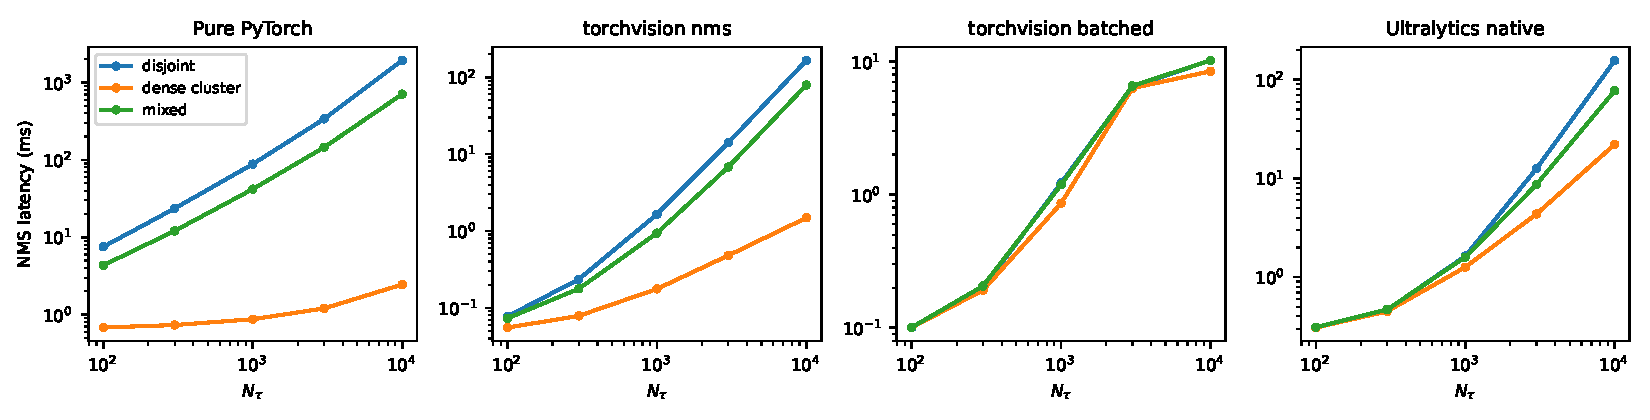
\includegraphics[width=\textwidth]{fig2_dose_response.pdf}
\caption{NMS latency against $\Ntau$ on the frequency-locked profile (10\,000-anchor grid, 80 classes, no cap) for four implementations and three box geometries. Lines are medians; shaded bands are 95\% bootstrap intervals over repetitions. Both axes are logarithmic.}
\label{fig:dose}
\end{figure*}
On the 2100-anchor head, pure-PyTorch NMS with 2100 disjoint candidates takes 215~ms against 0.748~ms with 10 candidates, a ratio of 287 (95\% confidence interval 286 to 288). Every end-to-end repetition of the pure-PyTorch pipeline with 2100 injected candidates (20 of 20; 95\% Wilson interval 0.84 to 1.00; median 254~ms) exceeds the 100~ms reference. Table~\ref{tab:dose} gives the ratio between $\Ntau=10^4$ and $\Ntau=10^2$ for all four implementations and three geometries: in all 12 cells the lower bound of the interval exceeds $1+\mathrm{MDE}$, but the magnitude ranges from 3.60-fold (pure PyTorch, dense cluster) to 2136-fold (torchvision \texttt{nms}, disjoint), almost three orders of magnitude across implementations and geometries (Fig.~\ref{fig:dose}).

\paragraph{Answer to RQ1.} NMS latency rises with $\Ntau$ in all 12 cells, by 3.60- to 2136-fold between $10^2$ and $10^4$ candidates.

\subsection{RQ2: implementation, geometry and top-$k$ cap}
\label{sec:q2}
% GENERATED by paper_en/tables_q3/make_tables_en.py -- DO NOT EDIT.
\begin{table*}[t]
\centering\small
\caption{Median NMS latency (ms) at $\Ntau=10^4$ (10\,000-anchor head, 80 classes) without a cap and with a top-300 cap, and the reduction factor (uncapped divided by capped; 95\% CI, bootstrap over repetitions).}
\label{tab:cap}
\begin{adjustbox}{max width=\textwidth}
\begin{tabular}{@{}llcccc@{}}
\toprule
Geometry & Implementation & No cap (ms) & Cap 300 (ms) & Reduction & 95\% CI \\
\midrule
Disjoint & pure PyTorch & 1929 & 23.4 & 82.5 & 82.2-82.7 \\
Disjoint & torchvision \texttt{nms} & 166 & 0.170 & 974 & 971-976 \\
Disjoint & torchvision batched & 10.2 & 0.194 & 52.5 & 52.4-52.6 \\
Disjoint & Ultralytics native & 157 & 0.457 & 342 & 337-346 \\
Mixed & pure PyTorch & 706 & 11.8 & 60.1 & 59.9-60.2 \\
Mixed & torchvision \texttt{nms} & 79.3 & 0.137 & 577 & 576-580 \\
Mixed & torchvision batched & 10.2 & 0.204 & 50.1 & 49.9-50.2 \\
Mixed & Ultralytics native & 77.7 & 0.471 & 165 & 164-168 \\
Dense cluster & pure PyTorch & 2.45 & 0.719 & 3.41 & 3.40-3.43 \\
Dense cluster & torchvision \texttt{nms} & 1.48 & 0.0752 & 19.7 & 19.6-19.8 \\
Dense cluster & torchvision batched & 8.45 & 0.193 & 43.7 & 43.6-43.8 \\
Dense cluster & Ultralytics native & 22.1 & 0.453 & 48.9 & 47.7-49.1 \\
\bottomrule
\end{tabular}
\end{adjustbox}
\end{table*}

\paragraph{Implementation and geometry at the same $\Ntau$ (H2).}
The medians of Table~\ref{tab:dose} show both effects at $\Ntau=10^4$. With mixed geometry the NMS stage takes 706~ms with the pure-PyTorch loop, 79.3~ms with torchvision \texttt{nms}, 77.7~ms with Ultralytics-native NMS and 10.2~ms with torchvision \texttt{batched\_nms}. Disjoint boxes against a dense cluster cost 1929 against 2.45~ms for the pure-PyTorch loop, 166 against 1.48~ms for torchvision \texttt{nms}, 157 against 22.1~ms for Ultralytics, and 10.2 against 8.45~ms for torchvision \texttt{batched\_nms}. At the same $\Ntau$, NMS cost can therefore differ by more than two orders of magnitude.

\paragraph{Top-$k$ cap (H3).}
Table~\ref{tab:cap} gives the median NMS latency at $\Ntau=10^4$ without a cap and with a cap of 300 candidates. The cap reduces NMS time in all 12 cells, but the reduction factor depends strongly on implementation and geometry: from 3.41-fold (pure PyTorch, dense cluster, where most boxes are suppressed early anyway) to 974-fold (torchvision \texttt{nms}, disjoint). Selecting the 300 highest scores belongs to the score-filter stage, which takes 0.20~ms at $\Ntau=10^4$ without a cap and 0.26~ms with the cap in the pure-PyTorch arm. A pipeline that caps the number of candidates before NMS blocks most of the benefit an increase of $\Ntau$ could bring, whatever the optimizer.

% GENERATED by paper_en/tables_q3/make_tables_en.py -- DO NOT EDIT.
\begin{table*}[t]
\centering\small
\caption{One-class candidate sets (10\,000-anchor head, no cap): median NMS latency (ms) of one class at $\Ntau=10^3$ and $10^4$, the same $10^4$ boxes spread over 80 classes, and two ratios of medians (descriptive). Same session design as Table~\ref{tab:dose}, 30 repetitions per cell.}
\label{tab:nc1}
\begin{adjustbox}{max width=\textwidth}
\begin{tabular}{@{}llccccc@{}}
\toprule
 & & \multicolumn{3}{c}{One class} & 80 classes & \\
\cmidrule(lr){3-5}\cmidrule(lr){6-6}
Implementation & Geometry & $10^3$ & $10^4$ & Ratio & $10^4$ & One / 80 classes \\
\midrule
pure PyTorch & disjoint & 87.7 & 1927 & 22.0 & 1923 & 1.00 \\
pure PyTorch & mixed & 41.5 & 704 & 17.0 & 703 & 1.00 \\
pure PyTorch & dense cluster & 0.766 & 2.42 & 3.16 & 2.44 & 0.991 \\
torchvision \texttt{nms} & disjoint & 1.65 & 165 & 99.9 & 166 & 0.996 \\
torchvision \texttt{nms} & mixed & 0.904 & 77.9 & 86.2 & 79.2 & 0.984 \\
torchvision \texttt{nms} & dense cluster & 0.134 & 1.53 & 11.5 & 1.49 & 1.03 \\
torchvision batched & disjoint & 1.67 & 173 & 103 & 10.2 & 17.0 \\
torchvision batched & mixed & 0.891 & 78.8 & 88.5 & 10.1 & 7.79 \\
torchvision batched & dense cluster & 0.164 & 1.87 & 11.4 & 8.41 & 0.222 \\
Ultralytics native & disjoint & 1.93 & 165 & 85.6 & 156 & 1.06 \\
Ultralytics native & mixed & 1.15 & 78.9 & 68.6 & 78.5 & 1.00 \\
Ultralytics native & dense cluster & 0.410 & 2.28 & 5.55 & 20.8 & 0.109 \\
\bottomrule
\end{tabular}
\end{adjustbox}
\end{table*}

\paragraph{Candidates concentrated in one class.}
The class-batched kernel is cheap with 80 classes because it suppresses each class separately. Table~\ref{tab:nc1} shows what happens when all candidates share one class (post hoc summary; the one-class grid has no $\Ntau=10^2$ level, so the preregistered $10^2$-to-$10^4$ ratio is replaced by the ratio between $10^3$ and $10^4$). NMS time grows with $\Ntau$ in all 12 one-class cells, 3.16- to 103-fold between $10^3$ and $10^4$. For the two class-agnostic implementations the class count makes no difference (one class against 80 classes: 0.99 to 1.00 for pure PyTorch, 0.98 to 1.03 for torchvision \texttt{nms}). For torchvision \texttt{batched\_nms} it does: with $10^4$ disjoint boxes one class takes 173~ms against 10.2~ms with 80 classes (17.0-fold), and with mixed geometry 78.8 against 10.1~ms (7.79-fold), the same cost as the class-agnostic kernel. With a dense cluster the one-class set is cheaper (0.222-fold), because the boxes of one class suppress each other; the same holds for Ultralytics native (0.11-fold).

\paragraph{Answer to RQ2.} Implementation and geometry change the cost of the same $\Ntau$ by more than two orders of magnitude, a top-300 cap reduces it 3.41- to 974-fold, and concentrating disjoint candidates in one class removes the advantage of the class-batched kernel (17-fold slower at $\Ntau=10^4$).

\subsection{RQ3: how many candidates slow end-to-end time, and do real attacks reach it}
\label{sec:q3}
% GENERATED by paper_en/tables_q3/make_tables_en.py -- DO NOT EDIT.
\begin{table*}[t]
\centering\small
\caption{Threshold $N^{*}$: the smallest grid level whose end-to-end ratio has a lower 95\% bound above $1+\mathrm{MDE}$ (full-pipeline injection, 20 images, no cap); ``$>$'': not reached. ``Measured'' uses the preregistered MDE (0.55\% at 320 px, 1.88\% at 640 px); ``MDE 0.69\%'' uses the repeated A/A. $^{\dagger}$Post hoc budget estimate. $^{\S}$Without flagged blocks (12/21 points flagged; 14 and 4 images remain).}
\label{tab:nstar}
\begin{adjustbox}{max width=\textwidth}
\begin{tabular}{@{}llccccccc@{}}
\toprule
 & & \multicolumn{3}{c}{320 px (grid 100, 300, 1000, 2100)} & \multicolumn{4}{c}{640 px (grid 300, 1000, 3000, 8400)} \\
\cmidrule(lr){3-5}\cmidrule(lr){6-9}
Implementation & Geometry & Measured & Predicted$^{\dagger}$ & Unflagged$^{\S}$ & Measured & MDE 0.69\% & Predicted$^{\dagger}$ & Unflagged$^{\S}$ \\
\midrule
pure PyTorch & disjoint & 100 & 100 & 100 & 300 & 300 & 300 & 300 \\
 & mixed & 100 & 100 & 100 & 300 & 300 & 300 & 300 \\
 & dense cluster & 300 & 100 & 300 & $>$8400 & $>$8400 & $>$8400 & $>$8400 \\
torchvision \texttt{nms} & disjoint & 1000 & 1000 & 2100 & 3000 & 3000 & 3000 & 3000 \\
 & mixed & 1000 & 1000 & 1000 & 8400 & 8400 & 3000 & 8400 \\
 & dense cluster & 1000 & 2100 & $>$2100 & $>$8400 & $>$8400 & $>$8400 & 8400 \\
torchvision batched & disjoint & 300 & 1000 & 300 & 1000 & 1000 & 3000 & 3000 \\
 & mixed & 1000 & 1000 & 1000 & 3000 & 1000 & 3000 & 3000 \\
 & dense cluster & 1000 & 1000 & 1000 & 3000 & 3000 & 3000 & 8400 \\
Ultralytics native & disjoint & 100 & 100 & 300 & 3000 & 3000 & 3000 & 3000 \\
 & mixed & 1000 & 100 & 1000 & 3000 & 3000 & 3000 & 3000 \\
 & dense cluster & 1000 & 100 & 1000 & 3000 & 3000 & 3000 & 3000 \\
\bottomrule
\end{tabular}
\end{adjustbox}
\end{table*}

\begin{figure*}[pos=!t]
\centering
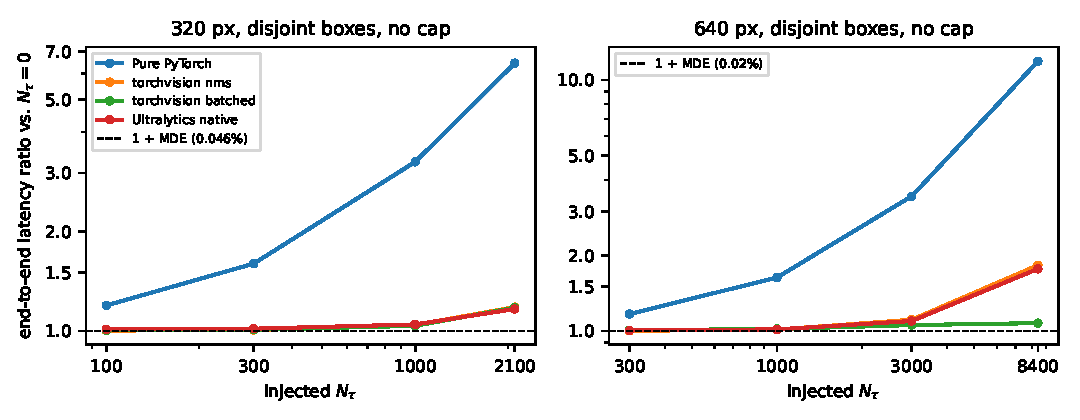
\includegraphics[width=\textwidth]{fig4_pipeline_nstar.pdf}
\caption{End-to-end time ratio against $\Ntau=0$ when disjoint candidates are injected into the full pipeline (20 images, no top-$k$ cap), at 320 px and 640 px. The dashed line is the preregistered end-to-end $1+\mathrm{MDE}$; shaded bands are 95\% bootstrap intervals over images. Both axes are logarithmic.}
\label{fig:nstar}
\end{figure*}
\paragraph{Threshold $N^{*}$ under full-pipeline injection (H4).}
We inject synthetic candidate sets into the full pipeline (a real forward pass on the image, then score filtering and NMS) for 20 held-out images, four implementations, three geometries, with and without a top-300 cap, at 320 px ($\Ntau$ from 0 to 2100) and 640 px ($\Ntau$ from 0 to 8400). The $\Ntau=0$ cell of each image is measured three times and used as the denominator. $N^{*}$ is the smallest grid level whose end-to-end ratio has a lower 95\% confidence bound (bootstrap over images) above $1+\mathrm{MDE}$. Design, endpoints and reading rule were preregistered. Pinning passed verification at the start and end of the session (1.00 and 1.00 effective cores), and 0 of 21 reference points were flagged (largest deviation 1.8\%).

With the low noise floor of the locked core, end-to-end time slows detectably from the lowest grid level in almost every cell: 100 candidates at 320 px for all four implementations and three geometries, and 300 candidates at 640 px in 11 of 12 cells, the exception being torchvision \texttt{nms} with a dense cluster (1000; Table~\ref{tab:nstar}, Fig.~\ref{fig:nstar}). $N^{*}$ is therefore an upper bound here: the true threshold may lie below the first grid level. The magnitudes still differ strongly. With disjoint boxes the pure-PyTorch pipeline is 6.45 times slower at 2100 candidates (320 px) and 11.9 times at 8400 candidates (640 px); with torchvision \texttt{nms} the same candidates make it 1.18 and 1.83 times slower, with torchvision \texttt{batched\_nms} 1.18 and 1.07 times, and with Ultralytics native 1.17 and 1.77 times. These are mean ratios; Table~\ref{tab:amdahl} aggregates the same cells as the mean log ratio against the median of the three $\Ntau=0$ cells, the computation used for the prediction, and its values differ slightly. The predicted column of Table~\ref{tab:nstar} is the post hoc budget estimate from the injection curves of the two detector heads with the clean $t_{\mathrm{total}}$ of the same session (39.7 to 39.8~ms at 320 px, 141~ms at 640 px). The in-session noise floor of the injection (second copy of the $\Ntau=0$ cell against the first) is 0.07-0.08\% at 320 px and 0.17-0.21\% at 640 px, higher than the MDE of the separate A/A; with this noise floor some thresholds could be one grid level higher. The top-300 cap blocks most of the increase for library kernels (at most 1.02 times at the largest $\Ntau$); the pure-PyTorch loop is still 1.60 times (320 px) and 1.17 times (640 px) slower at the largest $\Ntau$ with disjoint boxes, because 300 boxes are still many for a Python loop.

\paragraph{The threshold in milliseconds.}
\label{sec:threshold}
From $R \approx 1 + \Delta t_{\mathrm{NMS}}/t_{\mathrm{total}}$ (Section~\ref{sec:amdahl}), the NMS stage alone lifts the end-to-end ratio above $1+\mathrm{MDE}$ only when
\begin{equation}
\Delta t_{\mathrm{NMS}} > \Delta t^{*} = \mathrm{MDE} \times t_{\mathrm{total}} ,
\end{equation}
where $\mathrm{MDE}$ and $t_{\mathrm{total}}$ must share the end-to-end definition of the comparison. Increases in other stages draw on the same budget. The point threshold therefore applies to $\Delta t_{\mathrm{total}}$. The $N^{*}$ decision also requires the lower confidence bound of the ratio to exceed $1+\mathrm{MDE}$. For the patch session (clean $t_{\mathrm{total}}$ of 39.4~ms at 320 px and 142~ms at 640 px with torchvision; in-session MDE 0.20\% and 1.14\% from the two clean arms), $\Delta t^{*}$ is 0.080~ms at 320 px and 1.6~ms at 640 px (Table~\ref{tab:threshold}). The gradient baseline is the only condition that clearly raises $\Ntau$. With torchvision \texttt{nms} it adds 0.016~ms to the NMS stage (micro-benchmark), below $\Delta t^{*}$, so the budget model predicts an end-to-end ratio of only 1.0004; the measured ratio is 1.0018 (1.0009 to 1.0028), below $1+\mathrm{MDE}$. With the pure-PyTorch loop it adds 0.76~ms, above the $\Delta t^{*}$ of that arm (0.080~ms, from its own clean $t_{\mathrm{total}}$ of 40.3~ms); the model predicts 1.0189 and the measured ratio is 1.0203 (1.0177 to 1.0229), above $1+\mathrm{MDE}$.

% GENERATED by paper_en/tables_q3/make_tables_en.py -- DO NOT EDIT.
\begin{table*}[t]
\centering\small
\caption{Threshold $\Delta t^{*}$ for the end-to-end ratio to exceed the MDE in the patch session, and the gradient baseline (B4, 320 px, 100 images $\times$ 5 seeds). $t_{\mathrm{total}}$ and the MDE come from the two clean arms of the same session (prepared tensors). $\Delta t_{\mathrm{NMS}}$ is a micro-benchmark measurement; $R_{\mathrm{pred}}$ is the budget estimate and $R_{\mathrm{meas}}$ the end-to-end measurement.}
\label{tab:threshold}
\begin{adjustbox}{max width=\textwidth}
\begin{tabular}{@{}lcc@{}}
\toprule
 & torchvision \texttt{nms} & pure PyTorch \\
\midrule
Clean $t_{\mathrm{total}}$, 320 px (ms) & 39.4 & 40.3 \\
In-session end-to-end MDE, 320 px (\%) & 0.20 & 0.20 \\
Threshold $\Delta t^{*}=\mathrm{MDE}\times t_{\mathrm{total}}$, 320 px (ms) & 0.080 & 0.080 \\
Clean $t_{\mathrm{total}}$, 640 px (ms) & 142 & 144 \\
In-session end-to-end MDE, 640 px (\%) & 1.14 & 1.10 \\
Threshold $\Delta t^{*}=\mathrm{MDE}\times t_{\mathrm{total}}$, 640 px (ms) & 1.6 & 1.6 \\
\midrule
$\Delta t_{\mathrm{NMS}}$ of the gradient baseline, measured (ms) & 0.016 (0.013-0.019) & 0.76 (0.66-0.86) \\
Above $\Delta t^{*}$ (320 px) & no & yes \\
$R_{\mathrm{pred}} = 1+\Delta t_{\mathrm{NMS}}/t_{\mathrm{total}}$, budget estimate & 1.0004 & 1.0189 \\
$R_{\mathrm{meas}}$, measured (95\% CI) & 1.0018 (1.0009-1.0028) & 1.0203 (1.0177-1.0229) \\
\bottomrule
\end{tabular}
\end{adjustbox}
\end{table*}


% GENERATED by paper_en/tables_q3/make_tables_en.py -- DO NOT EDIT.
\begin{table*}[t]
\centering\small
\caption{Effect of the frozen patches relative to clean images of the same canvas, 100 images $\times$ 5 seeds, one drift-gated session (10/10 blocks accepted at the first attempt). All ratios are measured: mean over image $\times$ seed pairs, 95\% CI from a two-level bootstrap. NMS: torchvision, $\tau=0.01$. ``(above)'': lower bound $>1+\mathrm{MDE}$; MDE in-session (two clean arms), torchvision / pure PyTorch.}
\label{tab:patches}
\begin{adjustbox}{max width=\textwidth}
\begin{tabular}{@{}lcccccc@{}}
\toprule
Condition & $\Ntau$ ratio ($\tau$=0.01) & $\Ntau$ ratio ($\tau$=0.25) & NMS ratio & End-to-end, \texttt{nms} & End-to-end, pure PyTorch & MDE (\%) \\
\midrule
320 px, 64-px patch, $\tau_{\mathrm{obj}}$ 0.01 & 1.04 (0.99-1.10) & 0.94 (0.86-1.03) & 0.997 (0.985-1.009) & 1.0010 (1.0001-1.0019) & 1.0001 (0.9985-1.0017) & 0.20 / 0.20 \\
320 px, 64-px patch, $\tau_{\mathrm{obj}}$ 0.25 & 1.04 (0.99-1.09) & 0.95 (0.86-1.05) & 0.997 (0.984-1.008) & 1.0008 (0.9999-1.0017) & 0.9998 (0.9981-1.0014) & 0.20 / 0.20 \\
Random search (320 px) & 1.03 (0.98-1.08) & 0.95 (0.86-1.07) & 0.997 (0.984-1.009) & 1.0008 (0.9998-1.0017) & 1.0000 (0.9983-1.0016) & 0.20 / 0.20 \\
GA, centre placement (320 px) & 1.05 (0.99-1.10) & 0.90 (0.83-0.99) & 1.007 (0.995-1.019) & 1.0007 (0.9998-1.0017) & 1.0005 (0.9989-1.0021) & 0.20 / 0.20 \\
GA, random placement (320 px) & 1.06 (1.03-1.10) & 0.93 (0.87-0.97) & 1.005 (0.995-1.014) & 1.0009 (1.0000-1.0018) & 1.0011 (0.9997-1.0024) & 0.20 / 0.20 \\
Gradient ascent (320 px) & 2.39 (2.09-2.74) & 6.81 (4.72-9.44) & 1.247 (1.210-1.285) & 1.0018 (1.0009-1.0028) & 1.0203 (1.0177-1.0229) (above) & 0.20 / 0.20 \\
640 px, 128-px patch, $\tau_{\mathrm{obj}}$ 0.01 & 1.07 (1.00-1.16) & 0.94 (0.89-0.99) & 0.996 (0.976-1.013) & 0.9979 (0.9915-1.0041) & 0.9972 (0.9909-1.0035) & 1.14 / 1.10 \\
640 px, 64-px patch, $\tau_{\mathrm{obj}}$ 0.01 & 1.05 (1.02-1.08) & 0.96 (0.92-1.00) & 1.010 (1.001-1.018) & 1.0010 (0.9941-1.0080) & 1.0007 (0.9938-1.0075) & 1.14 / 1.10 \\
\bottomrule
\end{tabular}
\end{adjustbox}
\end{table*}

\begin{figure*}[pos=!t]
\centering
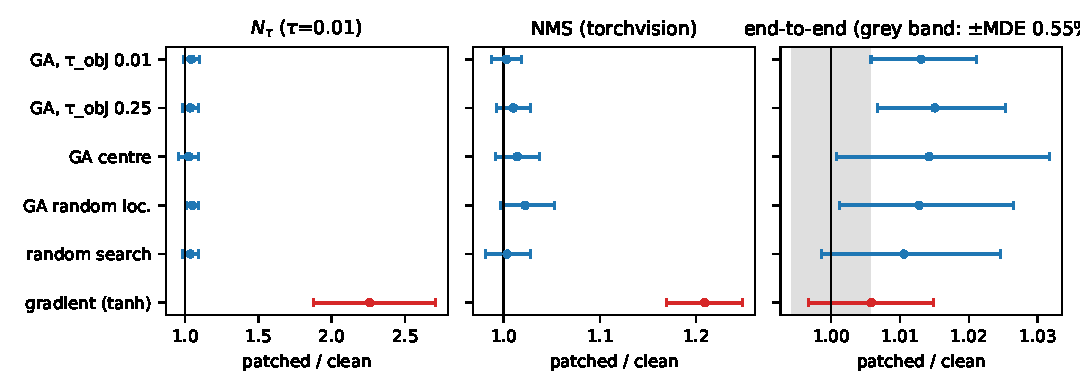
\includegraphics[width=\textwidth]{fig6_patch_effects.pdf}
\caption{Ratio between patched and clean images at 320 px, all measured in one drift-gated session, with 95\% two-level bootstrap intervals. Left and middle: $\Ntau$ and the NMS stage (torchvision). Right: end-to-end ratio (circles: torchvision \texttt{nms}; squares: pure PyTorch); the grey band is $\pm$ the in-session end-to-end MDE.}
\label{fig:patches}
\end{figure*}
\paragraph{Real patches.}
Every condition uses 100 held-out images and five patch seeds, measured in one session against two clean copies of each image on the same canvas (Table~\ref{tab:patches}). The genetic-algorithm patches do not raise $\Ntau$ appreciably (Fig.~\ref{fig:patches}): the median $\Ntau$ at $\tau=0.01$ goes from 86.5 (clean) to 85.5 and 85.0 for the two SG-GA conditions at 320 px, and for these and random search the intervals of the ratio contain 1 at both thresholds. Not every interval does. At $\tau=0.01$ the ratio lies slightly above 1 for random placement (1.06; 1.03 to 1.10) and for the 64-px patch at 640 px (1.05; 1.02 to 1.08). At $\tau=0.25$ it lies below 1 for centre placement (0.90; 0.83 to 0.99), random placement (0.93; 0.87 to 0.97) and the 128-px patch at 640 px (0.94; 0.89 to 0.99): at the higher threshold these patches reduce the candidate count. These medians are below the lowest grid level at which the injection already slows YOLOv8n at 320 px (100, Table~\ref{tab:nstar}); the comparison is only an order of magnitude, because $N^{*}$ is measured with synthetic candidates of controlled geometry. At 640 px the median $\Ntau$ rises from 119.0 to 134.0 (128-px patch) and 125.5 (64-px patch), also below the lowest 640-px level (300). The end-to-end measurements agree. For the seven GA, random-search and 640-px conditions the mean end-to-end ratio with torchvision \texttt{nms} is 0.9979 to 1.0010, and no lower bound exceeds $1+\mathrm{MDE}$ with either implementation. With a preregistered equivalence test (TOST, 90\% interval of the ratio inside $\pm1\%$), 15 of the 16 condition $\times$ implementation cells are equivalent to no change within 1\% (90\% bounds 0.9913 to 1.0059). Of the 14 GA, random-search and 640-px cells, 1 has a 95\% interval just above 1 (64-px SG-GA patch with torchvision, 1.0010; 1.0001 to 1.0019), an increase of 0.1\% that stays below the in-session MDE. The gradient baseline raises the median $\Ntau$ from 86.5 to 165.0 and the torchvision NMS stage 1.247-fold, yet the end-to-end ratio exceeds $1+\mathrm{MDE}$ only with the pure-PyTorch loop (1.0203; 90\% interval 1.0180 to 1.0224, not equivalent within 1\%), where NMS takes 2.3\% of clean end-to-end time against 0.13\% for torchvision. The budget estimate lies inside the 95\% interval of the measured ratio in 14 of 16 cells; the two misses are 320-px torchvision cells (64-px SG-GA patch and gradient baseline) where the measured ratio exceeds the prediction by 0.10 and 0.14 percentage points. A post hoc recount from stored historical data, which counts candidates only and measures no time, gives the same picture on five YOLO detectors (YOLOv8n, YOLOv8s, YOLO11n, YOLO11s, YOLOv12n) with five earlier SG-GA patches inserted: the $\Ntau$ ratio is 1.021 to 1.036 with intervals containing 1, and the median patched $\Ntau$ (85.0 to 104.0) stays at the level of clean images.

% GENERATED by paper_en/tables_q3/make_tables_en.py -- DO NOT EDIT.
\begin{table*}[t]
\centering\small
\caption{Adaptive variants of two whole-image attacks (YOLOv5s, 640 px, 50 images $\times$ 5 seeds, frequency-locked core). Median $\Ntau$ clean $\to$ perturbed and mean of the per-image $\Ntau$ ratios ($\tau=0.25$); end-to-end ratio (95\% CI, two-level bootstrap); ``above MDE'': lower bound $>1+\mathrm{MDE}$ of the session. $^{\dagger}$Post hoc: threshold $\Delta t^{*}$ and median NMS increase.}
\label{tab:attacks}
\begin{adjustbox}{max width=\textwidth}
\begin{tabular}{@{}lcclccccc@{}}
\toprule
Variant & $\Ntau$ clean $\to$ attack & $\Ntau$ ratio (95\% CI) & Implementation & End-to-end ratio (95\% CI) & MDE (\%) & Above MDE & $\Delta t^{*}$ (ms)$^{\dagger}$ & $\Delta t_{\mathrm{NMS}}$ (ms)$^{\dagger}$ \\
\midrule
Overload & 45.0 $\to$ 5578.5 & 389 (135-753) & torchvision \texttt{nms} & 1.018 (1.000-1.038) & 2.82 & no & 7.7 & 8.6 \\
 & &  & torchvision batched & 1.013 (0.993-1.033) & 2.82 & no & 7.7 & 5.9 \\
 & &  & Ultralytics native & 1.020 (1.001-1.040) & 2.80 & no & 7.7 & 8.4 \\
Phantom Sponges & 45.0 $\to$ 4811.5 & 340 (104-678) & torchvision \texttt{nms} & 1.016 (0.997-1.036) & 2.82 & no & 7.7 & 9.6 \\
 & &  & torchvision batched & 1.017 (0.998-1.036) & 2.82 & no & 7.7 & 9.5 \\
 & &  & Ultralytics native & 1.020 (1.001-1.040) & 2.80 & no & 7.7 & 10 \\
\bottomrule
\end{tabular}
\end{adjustbox}
\end{table*}

% GENERATED by paper_en/tables_q3/make_tables_en.py -- DO NOT EDIT.
\begin{table*}[t]
\centering\small
\caption{\textbf{Post hoc}, YOLOv5s (640 px): decomposition of the latency increase of the whole-image attack variants per image $\times$ seed pair (ms; 95\% CI, two-level bootstrap). The remainder is $\Delta t_{\mathrm{total}}-\Delta t_{\mathrm{NMS}}$; the raw records do not separate its stages.}
\label{tab:decomp}
\begin{adjustbox}{max width=\textwidth}
\begin{tabular}{@{}llcccc@{}}
\toprule
Variant & Implementation & $\Delta t_{\mathrm{total}}$ & $\Delta t_{\mathrm{NMS}}$ & Remainder & Remainder / $\Delta t_{\mathrm{total}}$ (\%) \\
\midrule
Overload & torchvision \texttt{nms} & 10.5 (6.8-14) & 5.24 (4.1-6.4) & 5.26 (1.8-8.7) & 50 \\
Overload & torchvision batched & 9.06 (5.3-13) & 4.91 (3.4-6.5) & 4.15 (0.82-7.6) & 46 \\
Overload & Ultralytics native & 10.7 (6.6-15) & 7.04 (5.7-8.4) & 3.66 ($-$0.18-7.6) & 34 \\
Phantom Sponges & torchvision \texttt{nms} & 10.0 (6.5-13) & 5.44 (4.3-6.6) & 4.58 (1.4-7.7) & 46 \\
Phantom Sponges & torchvision batched & 9.77 (6.0-14) & 5.99 (4.8-7.2) & 3.77 (0.31-7.9) & 39 \\
Phantom Sponges & Ultralytics native & 10.2 (6.0-14) & 6.86 (5.5-8.2) & 3.29 ($-$0.50-7.2) & 32 \\
\bottomrule
\end{tabular}
\end{adjustbox}
\end{table*}

\begin{figure*}[pos=!t]
\centering
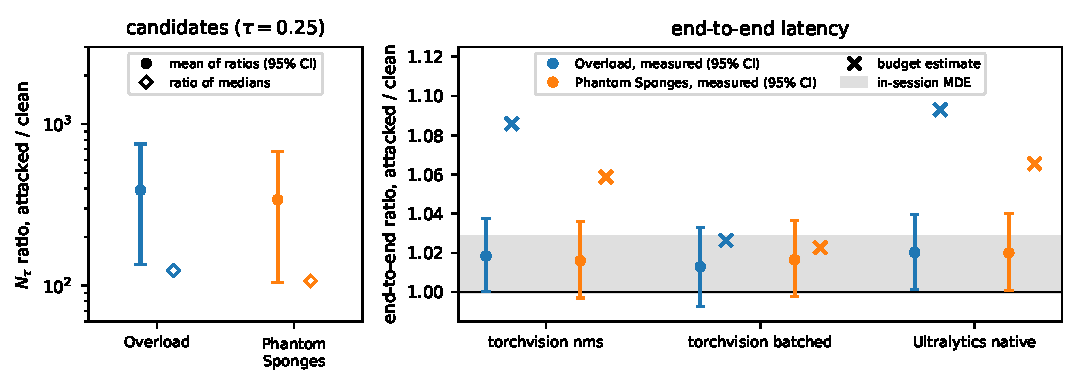
\includegraphics[width=\textwidth]{fig9_attacks.pdf}
\caption{Adaptive variants of two whole-image attacks (YOLOv5s, 640 px) on the frequency-locked core. Left: $\Ntau$ ratio ($\tau=0.25$) against clean images, logarithmic scale. Right: measured end-to-end ratio (dots, 95\% intervals) and the prediction of the preregistered Amdahl model (crosses) by NMS implementation; the grey band is the in-session MDE.}
\label{fig:attacks}
\end{figure*}
\paragraph{Variants of whole-image attacks.}
\label{sec:attacks}
The session passed pinning verification at the start and end (1.00 and 1.00) and 0 of 11 reference points were flagged (maximum deviation 1.9\%). The perturbations raise the median $\Ntau$ at $\tau=0.25$ from 45.0 to 5578.5 (Overload variant) and 4811.5 (Phantom Sponges variant), a ratio of medians of 124 and 107 (Table~\ref{tab:attacks}, Fig.~\ref{fig:attacks}). The mean of the per-image ratios is larger, 389 (95\% CI 135 to 753) and 340 (104 to 678), because images with few clean candidates pull it up; we report both statistics. At $\tau=0.01$ the median $\Ntau$ rises from 253.5 to 11674.0 and 14487.5. The NMS stage of the library kernels rises from a median of 0.047-0.29~ms to 6.0-11~ms, and that of the pure-PyTorch loop from 0.43~ms to 48-70~ms. End-to-end time with the library kernels rises only from a median of 273-274~ms to 281-285~ms: mean ratios of 1.013 to 1.020. The 95\% interval excludes 1 in 3 of the 6 cells (torchvision \texttt{nms} with the Overload variant and Ultralytics native with both), its lower bound exceeds $1+\mathrm{MDE}$ of the session (MDE 2.80-2.82\%) in none, and in a post hoc equivalence test the 90\% interval lies inside a $\pm5\%$ margin in all six cells but inside $\pm1\%$ in none. The MDE of this session is much larger than that of the A/A or the patch session; it is a property of the session, not of the attack, so these cells are not read as showing no effect. All comparisons here use the threshold of YOLOv5s itself, not the YOLOv8n threshold $N^{*}$: with the $t_{\mathrm{total}}$ and MDE of the YOLOv5s session, $\Delta t^{*}$ is 7.7~ms. The median increase of the NMS stage (5.9-10~ms) exceeds $\Delta t^{*}$ in five of six cells, yet the mean end-to-end increase (3.1 to 5.2~ms, post hoc) is below it in all six, with every 95\% interval containing 0. A decomposition per image $\times$ seed pair (Table~\ref{tab:decomp}, post hoc, no new measurement) accordingly finds a negative remainder, $-3.2$ to $-4.7$~ms, with every interval containing 0: in this session the end-to-end increase is not larger than the increase of the separately timed NMS stage, and the records give no evidence of a slowdown outside NMS. The NMS micro-benchmark and the NMS call inside the end-to-end timer need not cost the same (for example because the cache state after the forward pass differs; not tested), and the end-to-end differences are not resolved at this noise floor. This conclusion applies only to these variants, YOLOv5s and a single CPU core: on that configuration NMS still accounts for only 2.1-3.7\% of end-to-end time after the increase. Applying the Amdahl expression to the pure-PyTorch loop (end-to-end time not measured because of its cost) gives an inferred end-to-end increase of about 17-25\%; this is an inference from the model, not a measurement.

\paragraph{Answer to RQ3.} On YOLOv8n end-to-end time rises detectably from at most 100 injected candidates at 320 px for every implementation and from 300 at 640 px (1000 in one cell). The GA patches of the case study stay at the clean candidate level and change end-to-end time by less than 1\%; the gradient baseline slows the loop-based pipeline by 2.0\%; on YOLOv5s the whole-image variants raise the NMS stage above that model's $\Delta t^{*}$ in five of six cells, yet end-to-end time by only 1.3 to 2.0\%, below the noise floor of that session.

\subsection{RQ4: how accurate is a predictor based on $\Ntau$ alone}
\label{sec:q4}
\begin{figure*}[pos=!t]
\centering
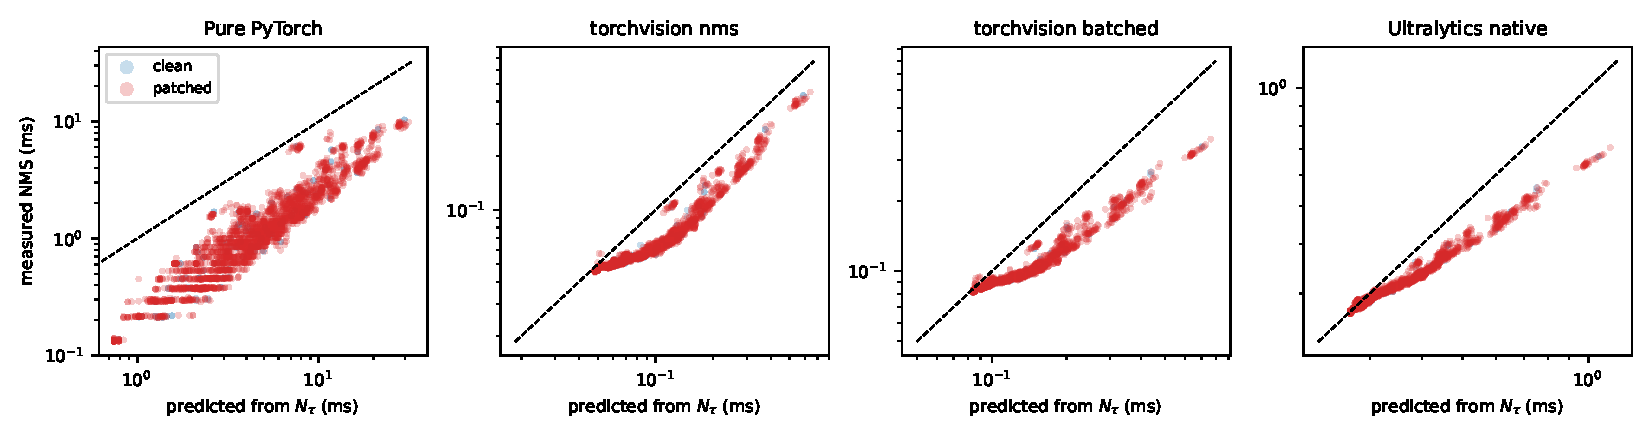
\includegraphics[width=\textwidth]{fig3_pred_vs_measured.pdf}
\caption{Measured NMS latency of real candidate sets ($\tau=0.01$, 320-px conditions) against the prediction from $\Ntau$ alone using the mixed-geometry dose-response curve, by implementation. The dashed line is equality. Blue points are clean images, red points patched images.}
\label{fig:pred}
\end{figure*}
\paragraph{NMS time of real candidate sets.}
For every measurement unit of the 320-px arms of the patch session with $\Ntau>0$, we predict $t_{\mathrm{NMS}}$ from $\Ntau$ alone by interpolating, on a log-log scale, the dose-response curve of the corresponding implementation (2100-anchor head, mixed geometry), and report the median and 90th percentile of $|\ln(t_{\mathrm{meas}}/t_{\mathrm{pred}})|$ (Fig.~\ref{fig:pred}; post hoc, as in the earlier laptop study, with no pass/fail threshold). Over 3200 measured points per implementation the median and 90th-percentile errors are 0.05 and 0.21 for Ultralytics native, 0.13 and 0.46 for torchvision batched, 0.30 and 0.58 for torchvision \texttt{nms}, and 1.45 and 1.78 for pure PyTorch (a typical error of about four-fold for the latter). The fraction of measured points that lie between the disjoint and the dense-cluster curves is 0.04 for Ultralytics native, 0.00 for torchvision batched, 0.36 for torchvision \texttt{nms} and 0.71 for pure PyTorch. Across clean images, the rank correlation of $\Ntau$ with NMS time is high (0.93 to 0.98 depending on the implementation), while for the within-image change caused by a patch it is lower (0.58 to 0.88 over the 320-px conditions): $\Ntau$ ranks cost across images better than it ranks the effect of an edit on one image. Both correlations are descriptive. On the whole-image attack variants, interpolation from $\Ntau$ alone errs by 0.42 to 1.83 (median log error), because candidates produced by the attacks overlap strongly and are suppressed faster than the synthetic mixed geometry.

% GENERATED by paper_en/tables_q3/make_tables_en.py -- DO NOT EDIT.
\begin{table*}[t]
\centering\small
\caption{Median error $|\ln(t_{\mathrm{meas}}/t_{\mathrm{pred}})|$ of $M_N$ and $M_{NK}$, fitted on the injection cells, on the real candidate sets of all arms of the patch session ($\tau=0.01$), and the difference $\Delta$ ($M_N$ minus $M_{NK}$) with a 95\% two-level bootstrap CI (images, units within images). $\Delta>0$ means that adding $K$ reduces the error.}
\label{tab:nk}
\begin{adjustbox}{max width=\textwidth}
\begin{tabular}{@{}lccc@{}}
\toprule
Implementation & $M_N$ & $M_{NK}$ & $\Delta$ (95\% CI) \\
\midrule
\multicolumn{4}{@{}l}{\textit{Real candidate sets of the patch session, \textbf{post hoc} (4397 units, 100 images)}} \\
pure PyTorch & 1.00 & 0.33 & 0.67 (0.55 to 0.74) \\
torchvision \texttt{nms} & 0.65 & 0.63 & 0.02 ($-$0.08 to 0.12) \\
torchvision batched & 0.70 & 2.07 & $-$1.37 ($-$1.47 to $-$1.26) \\
Ultralytics native & 0.46 & 2.48 & $-$2.02 ($-$2.12 to $-$1.91) \\
\bottomrule
\end{tabular}
\end{adjustbox}
\end{table*}

\paragraph{Does geometry explain the remaining error?}
\label{sec:nk}
We compare two log-linear models fitted per implementation on the cells of the synthetic injection: $M_N$, $\ln t_{\mathrm{NMS}} = a + b\ln\Ntau$, and $M_{NK}$, which adds a term $c\ln\max(K,1)$ where $K$ is the number of boxes kept by NMS. $K$ is a proxy for geometry but is known only after NMS has run, so $M_{NK}$ is a decomposition rather than a deployable predictor. The specification was fixed before fitting. Its preregistered confirmatory set, the 640-px candidate sets of the earlier laptop patch measurement, was not measured again; on the locked machine we evaluate the models on the real candidate sets of all arms of the patch session, which is post hoc (Table~\ref{tab:nk}). For the pure-PyTorch loop, adding $K$ cuts the error by about two thirds, as the cost model predicts; for torchvision \texttt{nms} no improvement is detected; for the two class-aware implementations $M_{NK}$ is clearly worse, because a model learned from synthetic sets (80 random classes) extrapolates poorly to the class distribution of real candidates. On the whole-image attack variants, $M_N$ errs by 0.27 to 0.61 and adding $K$ helps torchvision \texttt{nms} (difference 0.30; 0.22 to 0.35) and torchvision batched (0.16; 0.05 to 0.22) but not the other two. $\Ntau$ alone is not enough to predict NMS time, and a model calibrated entirely on synthetic candidates does not replace measurement on real candidates.

% GENERATED by paper_en/tables_q3/make_tables_en.py -- DO NOT EDIT.
\begin{table*}[t]
\centering\small
\caption{Budget estimate $R_{\mathrm{pred}} = 1+\Delta t_{\mathrm{NMS}}/t_{\mathrm{total}}$ against the measured ratio $R_{\mathrm{meas}}$; error is $|\ln(R_{\mathrm{meas}}/R_{\mathrm{pred}})|$. Part A (post hoc): full-pipeline injection, 156 cells, median error 0.012, 90th percentile 0.040; predicted and measured $N^{*}$ agree in 35/48 cells. Part B: whole-image attack variants on YOLOv5s, preregistered rule (upper 95\% bound of the median error $<0.05$); 3/6 cells pass.}
\label{tab:amdahl}
\begin{adjustbox}{max width=\textwidth}
\begin{tabular}{@{}lccccc@{}}
\toprule
 & $R_{\mathrm{pred}}$ & $R_{\mathrm{meas}}$ & Error (95\% CI) & $N^{*}$ predicted / measured & Rule \\
\midrule
\multicolumn{6}{@{}l}{\textit{A. Full-pipeline injection, \textbf{post hoc}; 320 px, disjoint boxes, no cap, $\Ntau=2100$}} \\
pure PyTorch & 6.44 & 6.57 & 0.020 & 100 / 100 & - \\
torchvision \texttt{nms} & 1.10 & 1.11 & 0.009 & 1000 / 1000 & - \\
torchvision batched & 1.14 & 1.20 & 0.056 & 1000 / 300 & - \\
Ultralytics native & 1.12 & 1.14 & 0.018 & 100 / 300 & - \\
\multicolumn{6}{@{}l}{\textit{A. Full-pipeline injection, \textbf{post hoc}; 640 px, disjoint boxes, no cap, $\Ntau=8400$}} \\
pure PyTorch & 10.5 & 10.9 & 0.035 & 300 / 300 & - \\
torchvision \texttt{nms} & 1.54 & 1.57 & 0.020 & 3000 / 3000 & - \\
torchvision batched & 1.06 & 1.09 & 0.023 & 3000 / 1000 & - \\
Ultralytics native & 1.56 & 1.58 & 0.015 & 3000 / 3000 & - \\
\midrule
\multicolumn{6}{@{}l}{\textit{B. Whole-image attack variants (YOLOv5s, 640 px), preregistered model and rule}} \\
Overload, torchvision \texttt{nms} & 1.067 & 1.034 & 0.046 (0.034-0.058) & - & \textbf{fail} \\
Overload, torchvision batched & 1.027 & 1.029 & 0.022 (0.017-0.028) & - & pass \\
Overload, Ultralytics native & 1.098 & 1.034 & 0.067 (0.049-0.088) & - & \textbf{fail} \\
Phantom Sponges, torchvision \texttt{nms} & 1.042 & 1.032 & 0.031 (0.024-0.038) & - & pass \\
Phantom Sponges, torchvision batched & 1.023 & 1.031 & 0.024 (0.019-0.030) & - & pass \\
Phantom Sponges, Ultralytics native & 1.065 & 1.033 & 0.044 (0.033-0.054) & - & \textbf{fail} \\
\bottomrule
\end{tabular}
\end{adjustbox}
\end{table*}

\paragraph{The Amdahl model for end-to-end time.}
On the full-pipeline injection, the Amdahl model with the injection curves (2100- and 8400-anchor heads) and the clean end-to-end time of the same session predicts the measured ratio with a median log error of 0.003 over 156 cells, and the predicted threshold equals the measured one in 40 of 48 cells (Table~\ref{tab:amdahl}; measured threshold computed with the model's aggregation, a sensitivity analysis; the primary threshold result is Table~\ref{tab:nstar}). This analysis is post hoc: the model was written after the injection had been seen on the earlier laptop data. On the patch session the estimate lies inside the 95\% interval of the measured end-to-end ratio in 14 of 16 cells (preregistered hypothesis, Section~\ref{sec:q3}). On the whole-image attack variants, with specification and rule fixed before measurement, the model fails the rule in all 6 cells: it predicts ratios of 1.023 to 1.093 where 1.013 to 1.020 are measured. There are two possible reasons, both from post hoc analysis. First, the synthetic mixed-geometry curve overestimates the NMS cost of real candidates (the interpolation error above). Second, even when the curve is replaced by the measured NMS time of the candidate set itself, the NMS-only model still misses (median log error 0.050-0.052), because the measured end-to-end increase is smaller than the separately timed NMS increase (Table~\ref{tab:decomp}). A further post hoc check compares the estimate with a constant no-change prediction, $R=1$. Because the measured ratios are small and noisy, that null prediction has a median log error of 0.043 to 0.046 on the same units, against 0.052 to 0.094 for the budget estimate; neither passes the rule in any cell. The skill of the budget estimate, one minus the ratio of the two errors, is $-1.16$ to $-0.14$, above zero in no cell, and the estimate is biased upwards in every cell (signed log bias 0.009 to 0.070). On effects this small and this noisy the budget estimate does not predict end-to-end time.

\paragraph{Answer to RQ4.} Without calibration to the implementation and geometry, $\Ntau$ mispredicts NMS time by up to about four-fold. The budget estimate is accurate on synthetic candidates and on the patch session, but on the real whole-image attacks it overestimates the end-to-end ratio and is worse than a no-change prediction in all six cells.

\section{Discussion}
\label{sec:discussion}
\subsection{What the measurements establish}
The measurements agree with the cost model of Section~\ref{sec:formal} in four respects. First, NMS latency grows with $\Ntau$ (H1): between $10^2$ and $10^4$ injected candidates it grows 3.60- to 2136-fold, and the growth is detected in all 12 cells against the MDE of the NMS stage (0.142\% and 0.182\%). Second, geometry determines how much it grows (H2): the loop-based implementation spends almost all of its time on kept boxes, so disjoint boxes cost more than two orders of magnitude more than a dense cluster of the same size. Third, the cap bounds the cost (H3): at $\Ntau=10^4$ a cap of 300 reduces NMS time 3.41-fold (pure PyTorch, dense cluster) to 974-fold (torchvision \texttt{nms}, disjoint). Fourth, the share of NMS in the pipeline decides whether a change in the NMS stage is visible end to end (H4): the same gradient patch adds 2.0\% to end-to-end time with the loop-based NMS (2.3\% of clean time) and 0.18\% with torchvision (0.13\%). What the cost model does not provide is the conversion from $\Ntau$ to milliseconds: a prediction based on $\Ntau$ alone errs four-fold for the loop-based implementation, although only by about 5\% for the Ultralytics implementation. The deadline result (every repetition of the pure-PyTorch pipeline with 2100 candidates exceeds 100~ms) shows only that the test bench can produce such an exceedance with that implementation, not that a deployed detector will miss a deadline.

\subsection{The budget estimate}
The budget estimate, $R \approx 1 + \Delta t_{\mathrm{NMS}}/t_{\mathrm{total}}$, is an Amdahl-type identity, useful as a quick check before measuring and not a theoretical contribution. On synthetic candidates it predicts the ratio with an error of about 0.3\% and the threshold $N^{*}$ correctly in most cells (post hoc), and on the patch session it lies inside the measured interval in 14 of 16 cells. On real whole-image attacks it fails the predefined criterion in all 6 cells and is worse than a no-change prediction: its inputs must be more accurate (an NMS curve with a geometry close to real candidates, and the NMS cost inside the pipeline rather than in isolation), and the effects it is asked to predict must be larger than the session noise floor before a pass is informative. An evaluator can still use it to see on which device an increase in $\Ntau$ could matter: it needs the NMS share on clean images and the NMS curve of the implementation in use. Conversely, a latency claim that states neither the NMS share nor the implementation cannot be checked.

\subsection{Why the measured attacks fall short, and when an attack would not}
The whole-image attack variants show the gap between the proxy and latency directly: on YOLOv5s, 640 px, one CPU core, the median candidate count grows more than a hundredfold (ratio of medians 107 and 124) and the NMS stage by more than an order of magnitude, but end-to-end time with the library kernels grows by only 1.3 to 2.0\%, because after the increase NMS still accounts for only 2.1 to 3.7\% of end-to-end time. On the locked core we find no part of the increase outside the NMS stage (Table~\ref{tab:decomp}). The earlier unlocked laptop measurement of the same perturbations had attributed a third to a half of a larger, about 3\% increase to other stages; that observation is not reproduced here, so it should not be read as a property of the attacks. A measurement that times the forward pass separately for clean and perturbed images would settle whether any stage outside NMS changes.

The case-study optimizer fails one step earlier: it does not raise $\Ntau$. In the stored training runs the genetic algorithm barely improves on random search with the same placement. A 64-px patch covers 4\% of a 320-px image, and a score threshold of 0.01 accepts every anchor with a little evidence of an object, so the candidate count is determined mostly by image content outside the patch. A gradient method can raise many anchors at once and increases the candidate count clearly (Table~\ref{tab:patches}), and it is the only patch that slows a pipeline measurably; a gradient-free search with 625 candidate evaluations cannot explore the space well enough. This is an observation about this optimizer and this budget, not a statement about gradient-free search in general.

The operational threshold applies to the added end-to-end time, $\Delta t_{\mathrm{total}}$. The budget estimate applies that threshold to the NMS contribution when the other stages are unchanged. From the expression we name three favourable configurations: an accelerated forward pass (GPU, neural accelerator) while NMS still runs sequentially, which shrinks the denominator; a loop-based NMS, where every kept box costs one iteration; and a pipeline without a top-$k$ cap before NMS. Our positive control has exactly the second and third (pure-PyTorch loop, no cap), and there, on YOLOv8n at 2100 disjoint candidates, end-to-end time is 6.45 times longer; on a low-noise core even the library kernels slow detectably from one hundred injected candidates, but only by a few percent. The accelerator case is a hypothesis for future work, not a result of this paper. Reported latency increases of NMS attacks are usually obtained with many boxes on a loop-based NMS kernel or on a GPU, on a specific edge device. Our results agree with the view that NMS latency attacks need a favourable combination of implementation, cap and geometry to matter, a view that EVADE argues from a different angle \cite{evade2025}. We do not reproduce the original experiments of the cited works and make no claim about other detectors or devices.

\subsection{Guidance, and what could change our conclusions}
For evaluators: report $\Ntau$ together with the implementation and cap, time stages separately, report the A/A noise floor, and state which deadline is being tested and why. For defenders: a cap on the number of candidates before NMS and a class-batched library kernel are settings that made the NMS stage insensitive to $\Ntau$ in our measurements, and they are cheap. The second holds only when candidates are spread over many classes: with $10^4$ disjoint boxes in one class the batched kernel is 17 times slower than with 80 classes and as slow as the class-agnostic kernel (Table~\ref{tab:nc1}), so the cap is the robust setting; top-$k$ selection itself costs a fraction of a millisecond. Caps and higher thresholds can also reduce accuracy, so the post-processing configuration is a trade-off, not a guarantee. For researchers proposing a latency attack: optimize latency, or a proxy whose relation to latency has been verified on the target pipeline, and report the effect against a noise floor.

A larger detector in which NMS is a larger share of the pipeline, an implementation with different constants, or a patch optimized with a latency term instead of $\Ntau$ could produce an end-to-end effect that this study does not detect. The end-to-end effects measured here are all within a few percent, so they are sensitive to the noise floor of each session: the whole-image session has a noise floor of 2.8\%, larger than the effects it measures, and a session with more repetitions per unit could resolve them.

\section{Threats to validity}
\label{sec:threats}
\paragraph{Scope of measurement.}
The detection study uses one desktop CPU, float32 inference on exactly one frequency-locked core; the absolute times and thresholds belong to this device. On this configuration the forward pass dominates (Table~\ref{tab:aa}), so the NMS share is small and, by the Amdahl model, end-to-end increases are compressed: the design is biased towards a ``no effect'' conclusion. Published latency-attack claims come from GPUs or edge devices with accelerators; the study does not reproduce those deployment conditions, so it does not refute those claims but provides a tool to check them. We attempted measurements on an Arm smartphone but could not verify core pinning under load, so no results are reported for that device. The Arm cross-check (Appendix~\ref{sec:pi3b}) uses a different model and workload on one undervolted board at 600~MHz; it qualifies total-time ratios only, has no qualified component breakdown, and is not a replication of the detection results.
\paragraph{Internal validity.}
Frequency, boost and the SMT sibling were locked and verified before and after every experiment, and no reference point of any session exceeded the 3\% drift flag, so drift is not a plausible explanation of the results; the machine ran a live operating system from memory, so other system services were still present. Timing noise is quantified by separate A/A runs and by an in-session noise floor when the design has two clean arms. These differ by design: 0.046\% end to end for the A/A at 320 px, 0.20\% for the patch session and 2.8\% for the whole-image session. The last is large relative to the effects it measures, and we have not established why it is larger than the others. The study repeats, with unchanged code, an earlier set of measurements on an unlocked laptop; the conclusions on candidate growth, caps and the patches agree, whereas the whole-image session differs in magnitude (about 3\% there, 1.3-2.0\% here) and in the share outside NMS. The two sets are kept separate and only the locked measurements are reported. The Amdahl model was written after the earlier full-pipeline injection had been seen; its tests on the patch session and the whole-image attacks are prospective.
\paragraph{Construct validity.}
Latency is measured on prepared tensors, excluding image decoding, camera capture and transport, and the end-to-end definition differs between the A/A (with resizing) and the other measurements; every threshold therefore uses the $t_{\mathrm{total}}$ of the same session. The 100~ms reference was chosen by the authors. Synthetic candidates have a controlled geometry that real candidates lack; the measurement on real attacks shows that the synthetic mixed geometry overestimates NMS cost. The Ultralytics post-processing has two cut-off mechanisms (library defaults, used unchanged): a limit of 30\,000 boxes passed to NMS, larger than every $\Ntau$ measured (at most $10^4$ in the injection and 25\,200 rows for YOLOv5s at 640 px), and a time limit of 2.05~s per image, against a largest median NMS time of 157~ms in the injection grid; 0 cells exceed this limit, so the mechanism cannot have been triggered.
\paragraph{External validity.}
The timing measurements use two one-stage detectors (YOLOv8n, YOLOv5s); for the newer YOLO models only candidate counts from historical data are available, without latency. One dataset family (COCO), 100 measured images and five patch seeds. NMS-free detectors, quantized models and accelerators are not covered; on a GPU or with an INT8 model the forward pass is faster, so the NMS share and the end-to-end effect of the same $\Ntau$ would be larger than measured here. The whole-image attacks are adaptive variants from public code, not reproductions of the original experiments, and require white-box access; patches are inserted digitally, without print-and-capture tests. The paper claims neither an attack stronger than previous work nor a denial of service on any deployed system.
\paragraph{Conclusion validity.}
Effects are read against the MDE; a confidence interval containing one, or an effect below the MDE, is reported as not detected at that sensitivity, not as equivalence. The threshold $N^{*}$ is read on a sparse grid and is sensitive to noise near the threshold; with the low noise floor of the locked core it falls on the first grid level in most cells and is then only an upper bound.

\section{Conclusion and future work}
\label{sec:conclusion}
On one frequency-locked CPU core, the cost of a given $\Ntau$ depends on the NMS implementation, the box geometry and the class distribution by more than two orders of magnitude. A top-300 cap reduced NMS time in all 12 implementation and geometry cells at $\Ntau=10^4$, whereas the class-batched kernel protected the pipeline only while candidates were spread over many classes: with $10^4$ disjoint candidates in one class it was 17 times slower than with 80 classes. With a loop-based NMS and no cap, 2100 injected candidates made YOLOv8n more than six times slower at 320 px, and on a low-noise core even library kernels slowed detectably from the lowest level tested (100 candidates at 320 px). With the optimizer and budget studied, Sponge Patch does not raise $\Ntau$ on YOLOv8n, and its measured end-to-end effect is equivalent to no change within 1\%; a white-box gradient patch slows the pipeline by 2.0\% only with a loop-based NMS. On YOLOv5s, adaptive variants after Overload and Phantom Sponges raise the median $\Ntau$ more than a hundredfold but end-to-end time by only 1.3 to 2.0\%, below the 2.8\% noise floor of that session, so that result is not conclusive. $\Ntau$ must therefore be calibrated to the implementation, geometry and class distribution before it is used as a latency proxy. The next steps are separate timing of every stage under attack with more repetitions, and the same protocol on accelerators, where the NMS share is expected to be larger.

\section*{Responsible release}
The tests process only data and models in an authorized research environment and do not disrupt any production service. The released artefacts are the measurement harness, the manifests, the synthetic-injection fixtures and the raw timing records; the optimized patches are not packaged as an attack tool, because they are not needed to support the argument about the limits of the proxy.

\section*{Data and code availability}
Code, manifests with file hashes and raw timing records, including those of rejected runs, are in the project repository \url{https://github.com/reikageisme/Sponge-patch-nms}, together with the preregistration files, the analysis and figure scripts and the hash of every patch. Numeric tables are generated from saved summary files, and a checking script compares the generated table text and source registry with a fresh build.

\section*{Declaration of generative AI use}
AI coding assistants (Claude Code and Codex) were used to help write and test the measurement harness, execute authorized experiments, and draft parts of the manuscript. The authors take responsibility for approving the hypotheses and endpoints, reviewing the measurements and source records, and the final content.

\section*{Funding and competing interests}
This research received no external funding; it is an independent research project of the authors. The authors declare no competing interests.

\appendix
\section{Cross-check on an Arm board where post-processing dominates}
\label{sec:pi3b}
\begin{table*}[pos=!t]
\centering\small
\caption{End-to-end latency ratios on the Raspberry Pi 3B at the declared 600~MHz clock (YOLOv8n-seg, 20 frozen image pairs; geometric means of per-image ratios, 95\% CI from 20\,000 resamples of images). The two sessions are separately preregistered conditions and are not pooled.}
\label{tab:pi3b}
\begin{adjustbox}{max width=\textwidth}
\begin{tabular}{@{}lcc@{}}
\toprule
Session & Attacked / clean & Capped / attacked \\
\midrule
Four threads, no USB device & 1.798 [1.747, 1.848] & 0.729 [0.713, 0.746] \\
One thread, idle USB SSD attached & 1.967 [1.902, 2.030] & 0.699 [0.682, 0.718] \\
\bottomrule
\end{tabular}
\end{adjustbox}
\end{table*}
\begin{figure*}[pos=!t]
\centering
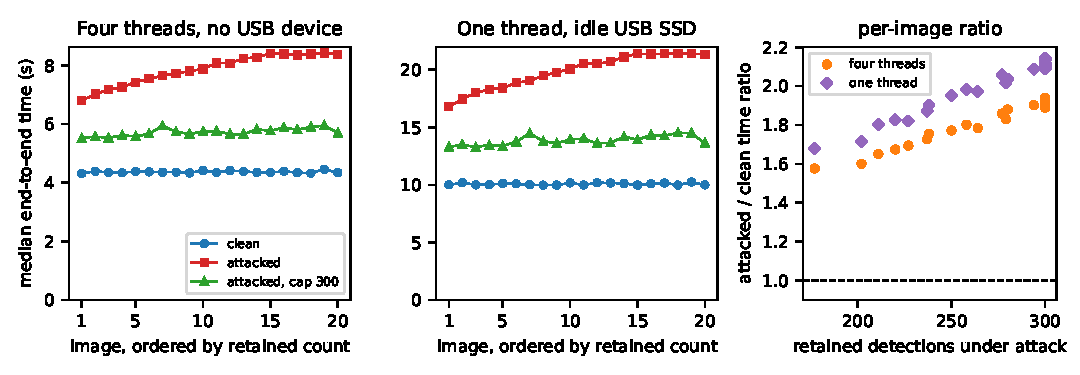
\includegraphics[width=\textwidth]{fig10_pi3b.pdf}
\caption{Raspberry Pi 3B at the declared 600~MHz clock (YOLOv8n-seg, 20 frozen image pairs). Left and middle: per-image median end-to-end time in the two qualified sessions, images ordered by the retained count under attack. Right: per-image attacked/clean ratio against the retained count. Descriptive; the sessions are not pooled.}
\label{fig:pi3b}
\end{figure*}
The detection results above come from a configuration in which the forward pass dominates. To observe the opposite regime on an Arm device, we replay, under separately preregistered protocols, 20 frozen whole-image perturbations (PGD, $L_\infty=16/255$, 100 steps, step size $2/255$) on YOLOv8n-seg, an instance-segmentation model whose post-processing builds one full-resolution mask per retained detection, so that post-processing work depends on the retained count as well as on $\Ntau$. The device is a Raspberry Pi 3B (four Cortex-A53 cores) whose firmware clamps the clock to 600~MHz because of undervoltage; this is the declared operating point, the sampled clocks are 600~MHz throughout, and no conversion to another clock is made. Inference is FP32 at $640\times640$ with confidence 0.25, IoU 0.45 and a fixed torchvision NMS backend, and the endpoint is the time from the prepared tensor to the returned native masks. On this model the perturbations raise the median retained count from 2.5 to 270, and the counts on the board match those on the laptop for all 20 pairs.

Table~\ref{tab:pi3b} gives the two sessions that pass every preregistered quality gate (load checks, reference drift, swap disabled, A/A noise floor, configuration restoration). With four threads pinned to the four cores (720 trials, none of 22 reference points flagged, A/A ratio 0.9990), attacked inputs take 1.798 times as long as clean ones (95\% CI 1.747 to 1.848; exact sign-flip $p=0.00000191$). With one pinned core the ratio is 1.967 (1.902 to 2.030; all 20 images positive), and the median total is 10.05~s clean against 20.30~s attacked. The single-core session is a distinct declared condition: an idle, separately powered and unmounted USB SSD was attached, its written-sector counters stayed at zero for the whole session, and its result is not pooled with the four-thread one. In the four-thread session the median per-image share of the forward pass falls from 98.6\% on clean inputs to 54.0\% on perturbed inputs: after the attack almost half of the time is post-processing, the regime in which H4 allows a detectable end-to-end effect. Limiting the candidates passed to NMS to 300 reduces the attacked total to 0.729 (0.713 to 0.746) and 0.699 (0.682 to 0.718) of its uncapped value, in the direction of H3. Fig.~\ref{fig:pi3b} shows the per-image times: the clean time is nearly constant across images, whereas the attacked time grows with the number of retained detections (177 to 300 per image), giving per-image ratios of 1.577 to 1.939 with four threads and 1.678 to 2.144 with one thread. This across-image trend is descriptive.

The result has clear limits. The component session that should separate NMS from mask construction completed 705 trials but failed its NMS precision gates (A/A ratio 0.9476, log-MDE 0.1652), while its mask control passed (0.9941, log-MDE 0.0271); the joint gate therefore fails, and we do not attribute the slowdown to NMS, to mask construction or to any split between them. Two earlier protocols on the same board failed their swap or pilot-precision gates and are kept as rejected runs. The 20 pairs are frozen inputs reused across sessions, not an independent cohort; the intervals resample images only and do not cover perturbation seeds, boards or supply conditions. The numbers describe one undervolted board and a different model and workload from the detection study, so their magnitude is not comparable with it; they do not transfer to a 1.2~GHz operating point and do not establish a missed service deadline or a denial of service.

\section{Deviations and negative results}
\label{app:dev}
\begin{table*}[pos=!t]
\centering\small
\caption{Deviations and negative results of the study. All raw records, including rejected runs, are kept in the repository.}
\label{tab:dev}
\begin{tabularx}{\textwidth}{@{}p{3.3cm}X@{}}
\toprule
Item & What happened and how it was handled \\
\midrule
Change of test bench & The reported timing results replace those of an earlier study on an unlocked laptop (Windows, frequency and turbo free, SMT sibling not blocked), after an internal review asked for a frequency-locked machine. Every timing experiment was repeated with unchanged code under a new preregistration; the laptop numbers are kept in the repository and are not pooled with the reported ones. \\
Replication runs & A path error in the run script stopped the first smoke test before any measurement, and missing Python packages (not used inside any timed region) stopped two experiments at import; both were fixed and recorded before the main session, which ran once per experiment. Every reference point of every session stayed below the 3\% drift flag, and all ten blocks of the drift-gated patch session were accepted at the first attempt. \\
Analysis adaptations & The analysis script of the patch session read drift records of a format that the new drift gate does not write; a wrapper converts the gate records without changing the analysis. The one-class grid has no $\Ntau=10^2$ level, so its preregistered $10^2$-to-$10^4$ ratio is replaced by the $10^3$-to-$10^4$ ratio and the one-class/80-class ratio (post hoc). The confirmatory set of the $M_N$/$M_{NK}$ comparison (laptop patch run) was not re-measured; the models are evaluated post hoc on the candidate sets of the patch session. \\
Earlier laptop study & Its first patch measurement called the patch insertion inside the end-to-end timer of patched arms only, and its corrected re-measurement was rejected for drift; on the laptop the end-to-end patch effect was therefore only a budget estimate. Two early A/A attempts, a backend defect at $\Ntau=6$ and a heavily disturbed 640-px A/A were handled there as recorded in the repository. \\
Amdahl model & The model was written after the full-pipeline injection of the laptop study had been seen; its comparison on the injection is post hoc, and the tests on the patch session and the whole-image attacks are prospective. \\
\bottomrule
\end{tabularx}
\end{table*}

\FloatBarrier
\bibliographystyle{apa7num}
\bibliography{references}
\end{document}
